\documentclass[11pt,a4paper]{article}
\usepackage[margin=24mm]{geometry}
% Japanese reference translation: compile with LuaLaTeX (luatexja).
\usepackage{luatexja}
\usepackage[haranoaji]{luatexja-preset}
\usepackage{microtype}
\usepackage{amsmath,amssymb,amsthm,mathtools}
\usepackage{booktabs,tabularx,longtable,array}
\usepackage{graphicx,xcolor,xurl}
\usepackage[round,authoryear]{natbib}
\usepackage[hidelinks,breaklinks]{hyperref}
\hypersetup{
 pdftitle={回転楕円体上の錐体積重み付き角度エネルギーの停留点と鞍点円の数え上げ（日本語参考訳）},
 pdfauthor={Katsushi Furuta},
 pdfsubject={統合研究稿 v0.5.6 の日本語参考訳：体積保存回転楕円体上の停留集合の条件付き分類},
 pdfkeywords={spheroid, stationary set, cone volume measure, radial Gauss map, Morse-Bott, validated numerics}
}
\usepackage{enumitem}
\setlist{itemsep=3pt,topsep=5pt}
\setlength{\emergencystretch}{3em}
\setlength{\parskip}{3pt}
\setlength{\parindent}{1.3em}
\numberwithin{equation}{section}
\newtheoremstyle{jplain}{\topsep}{\topsep}{\normalfont}{}{\bfseries}{}{1em}{}
\theoremstyle{jplain}
\newtheorem{theorem}{定理}[section]
\newtheorem{proposition}[theorem]{命題}
\newtheorem{lemma}[theorem]{補題}
\newtheorem{corollary}[theorem]{系}
\newtheorem{claim}[theorem]{主張}
\newtheorem{computationalassertion}{計算主張}
\renewcommand{\thecomputationalassertion}{C\arabic{computationalassertion}}
\theoremstyle{jplain}
\newtheorem{definition}[theorem]{定義}
\newtheorem{conjecture}[theorem]{予想}
\theoremstyle{jplain}
\newtheorem{remark}[theorem]{注意}
\newcommand{\av}[1]{\left\langle #1\right\rangle}
\newcommand{\E}{\widehat E}
\newcommand{\cO}{c_{\mathrm o}}
\newcommand{\bO}{b_{\mathrm o}}
\newcommand{\cP}{c_{\mathrm p}}
\newcommand{\bP}{b_{\mathrm p}}
\newcommand{\vol}{\operatorname{Vol}}
\newcommand{\diag}{\operatorname{diag}}
\newcommand{\tr}{\operatorname{tr}}
\newcommand{\R}{\mathbb R}
\newcommand{\B}{B^3}
\newcommand{\Sph}{S^2}
\newcommand{\dd}{\,d}
\newcommand{\one}{\mathbf 1}
\renewcommand{\proofname}{証明}
\renewcommand{\contentsname}{目次}
\renewcommand{\refname}{参考文献}
\renewcommand{\tablename}{表}
\renewcommand{\figurename}{図}
\renewcommand{\abstractname}{要旨}
\title{回転楕円体上の錐体積重み付き角度エネルギーの\\停留点と鞍点円の数え上げ}
\author{古田 勝士（Katsushi Furuta）\\DAYBREAK（独立研究）\\\small ORCID: 0009-0005-3129-8043}
\date{統合研究稿 v0.5.6（2026年11月23日）の日本語参考訳}
\begin{document}
\maketitle
\begin{center}\small
\fbox{\parbox{.92\linewidth}{本稿は、英語版 \emph{Counting stationary points and saddle circles of a cone-volume-weighted angle energy on spheroids}（統合研究稿 v0.5.6、PDF の SHA-256 は \texttt{136d61aa\ldots3fb35}）の日本語参考訳である。正本は英語版であり、食い違いがあれば英語版に従う。数式、番号、文献、リンクは英語版のままである。翻訳は Claude Code（Anthropic）による（2026年11月23日）。著者による校閲は済んでいない。}}
\end{center}
\begin{abstract}
数値探索によって、扁長回転楕円体の中に赤道上の鞍点円が見つかる。第二の円や、赤道から外れた臨界点を、どうすれば排除できるか。錐体積に関して平均した動径–法線角の二乗について、停留集合の図式の全体を、六つの明示的な計算主張に帰着する。とくに、回転によって臨界軌道の全体が一つのスカラーの根になり、接方向の四階微分がその動径方向の交差を決める。探索的な横断符号の被覆では、31,340 枚の葉のうち 21,254 枚が未決のまま残った。接方向の四階微分の二つの表示から、軸比 2 から 5 までの赤道上の 731 個の箱すべてで、負の上界が得られる。第二の実装は、同じ箱を 1,043 個の終端片で包囲する。すると、動径方向の狭義単調性によって、鞍点円の存在は二つの端点の符号に帰着する。解析的には、球では内部の停留点はただ一つで、それは最小点である。また $0<\lambda\le 1/32$ では、内部の停留点は中心にある指数 1 の鞍点だけであり、全勾配の境界トレースは零点を持たない。体積保存族の全体にわたって、解析的な端点の評価と六つの名指しした入力から、中心、軸上の鞍点の対、赤道の鞍点円、および境界の勾配トレースに関わる四つの遷移が得られる。
\end{abstract}
\noindent\textbf{キーワード：} 回転楕円体；停留集合；錐体積測度；動径 Gauss 写像；Morse--Bott 臨界多様体；精度保証付き数値計算。

\section*{主結果と現状}
\noindent\textbf{条件付き分類。}
計算主張 C1--C6 を仮定すると、$\lambda>0$ の族全体にわたって、内部の停留成分は、
中心、$\cO<\lambda<\bO$ における指数 1 の鞍点の軸上の対、
および $\bP<\lambda<\cP$ における赤道の Morse--Bott 鞍点円だけである。
中心は $\cO$ と $\cP$ で型を変える。
全勾配の境界トレースが消えるのは、$\lambda=\bO$ のときの両極と、
$\lambda=\bP$ のときの赤道円の上だけである。
正確な閾値、指数、排除は、
定理~\ref{thm:classification} と表~\ref{tab:classification} にある。
閾値の近似値は $\cO\approx0.408$、$\bO\approx0.644$、
$\bP\approx2.065$、$\cP\approx4.724$ である（表~\ref{tab:critical}）。

\noindent\textbf{検証の現状。}
解析的な議論は書き下してあり、計算主張 C1--C6 は、
出典の記録、実装、点検の及ぶ範囲を特定したうえで、明示的に述べてある。
本稿そのものは、これらの計算上の入力の認証を完了させるものでも、
その位置づけを改めるものでもない。族全体の分類は、
C1--C6 を条件としたままである。本稿は証明の整備段階の原稿であり、
投稿できる段階の認証の主張ではない。著者の検証記録
（記録 V24、2026年11月16日；
\href{https://github.com/cotaxxxx/bg-spheroid-family/blob/127be52046e9498d1306fe3d35c3e02e91c636de/runs/2026-11-16/D_OB_GLOBAL_CLOSED_V24/JUDGE_RULING_D_OB_GLOBAL_CLOSED_20261116.md}{固定された検証記録}；
第~\ref{sec:availability}節を見よ）では、扁平の窓
$\lambda\in[2/5,33/50]$ の検証が完了している。これとは別に行った AI 支援の
プロジェクト監査が、組み立てと、計算の出典の参照を点検した。
裏づけとなる区間計算は、選んだ箱の独立な再計算と、
整数による厳密な被覆の検査によって点検しており、
個々の範囲は \path{CURRENT_REPRODUCTION_v0_5_4.md} に述べてある。
これらの点検は、C1--C6 の完全な再実行ではない。
命題~\ref{prop:sphere} は、球の場合 $\lambda=1$ を、
計算上の入力なしに証明する。今回の編集上の
改訂は、数学的な主張も、計算上の入力の位置づけも変えない。
\clearpage
\tableofcontents
\clearpage
\section{問題とその背景}\label{sec:introduction}

縦横比$\lambda=3$において、数値探索は参照座標で$0.823938$付近に停留半径を見出す。その点を回転させると円が得られる。第二の半径、あるいは赤道面の外の停留点を排除するものは何か。正規化した動径方向微分$H$の探索的な三次元被覆では、31,340個の終端の箱のうち21,254個で符号が分離されないまま残った。これらの箱は、停留点を数えるものでも、分類定理の破綻を数えるものでもない。これらは、第一の実験が答えられなかった問いがどれであるかを正確に教えてくれる。

第二の実験は、赤道から離れたところで鉛直方向微分を用い、次いで赤道上でスカラーの交差を数えた。本稿で報告する第三の実験は、点での値が示唆するより強い赤道上の単調性が、領域全体の包囲のもとでも成り立つかを問う。第一の実験は中実の子午線領域と形状区間を被覆し、第三の実験は赤道半径と形状のみを被覆する。各実験はそれぞれ自身の領域の上で用いる。これらを合わせると、族全体に対する問いが動機づけられる：停留成分の個数、次元、型は形状とともにどのように変化するか。

極値を与える中心はこの問いの一部である。鞍点も重要である。鞍点は、極値を選ぶ選択規則では捨てられてしまう停留構造の変化を記録するからである。回転楕円体はとりわけ扱いやすい試験例を与える：球の停留点は一つであるが、回転対称性は、中心から離れたところに、孤立した軸上の臨界点の対と円状の臨界多様体の両方を許す。本分類の目的は、これらの集合がいつ現れるかを決定し、非コンパクトな形状区間にわたって追加の成分を排除することである。

% Internal, AI-assisted research draft.  Author verification and the target
% journal's current AI policy must be resolved before submission.
% Bibliography keys are defined in ../references_additions.bib.
\subsection{関連する中心の問題と動機}
\label{subsec:related-centers}

物体の内部に特別な点を選ぶことには、変分的な観点からの相当な
歴史がある。Moszy\'nskaの動径中心は、選んだ点からの動径距離の関数の球面
平均を最大化することで定義され、
凸体に対しては、凹かつ狭義単調増加な平均化プロファイルが一意的な
最大点を与える\citep{moszynska2000selectors}。O'Haraは、Rieszポテンシャルと
その正則化から一般化された中心を展開している
\citep{ohara2012renormalization}。ポテンシャルの次数を$\beta$と書くと、
正則化していない式は次のとおりである：
\[
 V_{\Omega}^{(\beta)}(p)
   =\int_{\Omega}|x-p|^{\beta-n}\,dx,\qquad \beta>0.
\]
問題となる極値は次数に依存し、$\beta=n$では対数による置き換えが、
非正の次数では正則化が伴う。滑らかな凸体
$K\subset\mathbb R^3$と$0<\beta<3$に対して、このRieszポテンシャルの発散定理による
表示は次のとおりである：
\[
 V_{K}^{(\beta)}(p)
  =\frac{1}{\beta}\int_{\partial K}|x-p|^{\beta-3}
       (x-p)\cdot n(x)\,dA(x).
\]
幾何学的な因子$(x-p)\cdot n(x)\,dA(x)$は、まさに
以下で用いる基点に依存する錐体積の重みである。O'Haraのポテンシャルは
これに距離のべきを掛けて、極値を与える
中心を選ぶのに対し、本論文のエネルギーはこれに、動径方向と外向き法線の間の
角の二乗を掛け、
回転楕円体の軸比が変わるときのすべての停留成分を調べる。これらの構成は、
基点そのものを幾何学的汎関数の変数として
扱うことの自然な先例を与える。

これらの文献における一意性は、汎関数と物体の幾何の
両方に依存する。O'Haraは、与えられた各ポテンシャル次数において、非球面性が十分小さいとき、極値を与えるRieszポテンシャル中心の
一意性を証明している\citep{ohara2022nearly}。Sakataは、
狭義単調減少な動径核をもつポテンシャルの最大点を研究し、
一意性のための追加の十分条件を証明し、
最大点が二つ以上ある例を調べている\citep{sakata2016uniqueness}。とくに、平面の円環
$A=\{y\in\mathbb R^2:1\leq|y|\leq2\}$に対しては、その
$r^{-1/2}$ポテンシャル中心の集合は円であり、円板の和集合は
そのような中心を二つもちうる。これらの例は非凸な平面領域であるが、
本論文の円はこれに対し、凸な三次元の扁長
回転楕円体の内部における角度エネルギーのMorse--Bott\emph{鞍点}集合として
現れる。これらの例は、極値集合の構造に
注意深く目を向ける動機となるが、ここで考える角度
汎関数の停留集合を分類するものではない。また、選ばれた大域的
極値点の一意性は、それだけでは、別の
汎関数のすべての臨界点を記述するものでもない。

我々の問題は、$p$から境界点$x$へ向かう方向と
$x$における外向き法線との間の角の二乗を、次の
基点に依存する確率測度で平均したものに関わる：
\[
 d\mu_{K,p}(x)
   =\frac{(x-p)\cdot n(x)}{3\,\operatorname{Vol}(K)}\,dA(x)
   \qquad (p\in\operatorname{int}K).
\]
したがって、この定義には、視線
方向と重みに加えて法線場も関わる。我々は、このエネルギーを動径核の
体積ポテンシャルと同一視せず、これに対して前述の一意性定理を援用することもしない。
その代わりに、$p$に関する導関数が
消える集合の全体を調べる。回転楕円体族については、パラメータ$\lambda$は体積を固定して形状を
変えるものであり、Riesz核の次数$\beta$ではない。目的は、
中心の臨界点、軸上の対、および回転対称な
臨界円が、それらの退化と境界への接近も含めて、
一つの停留集合の図式にどのように収まるかを決定することである。

動径Gauss写像は、凸体の境界上で、動径方向に外向き
法線を対応させる。Gauss像
問題におけるその役割は、B\"or\"oczky, Lutwak, Yang, Zhang, Zhaoによって研究されている
\citep{boroczky2020gaussimage}。我々の汎関数にも、これと同じ
動径–法線の対応が現れるが、基点$p$は物体の内部を
動く。比較のために述べると、BertrandによるGauss曲率
指定問題の最適輸送による定式化では、（同論文の式~(6)において）外向き法線
$n$と動径方向$u$の間の角度コスト
$c(n,u)=-\log\cos d_{\mathbb S^2}(n,u)$が用いられる\citep{bertrand2016gauss}。ここでは
コストはその代わりに角の二乗$d_{\mathbb S^2}(n,u)^2$であり、これを
錐体積の確率測度に関して平均するが、その停留点を分類するためにGauss像の定理や
曲率指定の定理を援用することはしない。

熱流の中心は、関連するが別種の比較対象を与える。
MagnaniniとSakaguchiは、温度が
$u_t=\Delta u$を満たし、初期温度が$1$、境界温度が$0$である有界な伝導体を研究している
\citep{magnaniniSakaguchi2004hotspot}。ホットスポットとは$u(\,\cdot\,,t)$を最大にする点であり、
彼らの定常ホットスポットの問題は、同じ点がすべての正の時刻において
最大点であり続けるかどうかを問う。そこで述べられている凸な伝導体の問題では、
固定した各正の時刻において、空間的な臨界点はただ一つである。
ここで調べる条件は、固定した各形状における$d_p E_\lambda=0$であり、
極値点だけでなく鞍点も含む。その定義に
熱の時間発展は現れない。したがって、角度の
問題に鞍点円が現れることは、ホットスポットの一意性の結果から導かれることも、それと矛盾することもない。

非有界な形状の範囲にわたってそのような図式を確立するには、
解析的な簡約と数値的な検証とを結ぶものが必要である。この結びつきは、
計算機援用証明の確立された実践に属するものであり、
Tuckerによる常微分方程式の厳密な解析がその例であって、彼による精度保証付き
数値計算の解説およびG\'omez-Serranoの概説において説明されている
\citep{tucker2002rigorous,tucker2011validated,gomezSerrano2019survey}。
JohanssonのArbは、任意精度の
中心半径型演算の標準的な実装を提供し\citep{johansson2017arb}、彼の後の
論文は、ボール演算における厳密な数値積分を記述している
\citep{johansson2018integration}。演算による包囲
だけでは、特定の積分核の正しさや
領域被覆の完全性は確立されない。証明は、どの
不等式が排除、存在、一意性、および型を導くのか、また
有限被覆が解析的な端点領域とどのように接続するのかも、明示しなければならない。我々は、
精度保証付き数値計算の枠内での、公式、
包囲、および検査のこの問題固有の組織化を\emph{GeoEnclosure}と呼ぶ。


区間Newton判定とKrawczyk判定は、箱の内部の正則な根を分離できる\citep{intervalNewton}。分枝刈り込み型の解法は、局所的な判定と孤立根の大域的な探索とを組み合わせる\citep{branchPrune}。半径多項式法は、Newton型写像が縮小写像となる球を見つけることで、局所一意性を証明できる\citep{radiiContinuation}。停留円においては、全勾配のJacobianが軌道に沿って至るところ特異であり、軌道のどの点も孤立していない。回転によって軌道座標が取り除かれ、スカラーの分離が意味をもつようになる。ここでの問題固有の寄与は、デカルト座標での接方向の四階導関数から動径方向の交差を復元すること、および直接の微分が接触に出会うところで弦Hessianの差に切り替えることである。被覆と分離の原理そのものは標準的である。

\paragraph{このエネルギーに関する先行研究。}
著者による以前の球に関する原稿は、球に対する同じ
停留点・最小点の結果を与えているが\citep{furutaSphere}、本論文の
命題~\ref{prop:sphere}の証明は自己完結しており、
その原稿に依拠しない。Furutaによる以前の扁長側の局所
分岐の計算\citep{furutaProlate}は、中心における赤道方向の二次係数の零点を、Arbによる端点評価によって
$[4.72438340452113340672,4.72438340452113340673]$の中に
分離している。その軸比は本論文の$\lambda$である。横断方向の長さの単位を変えても、二次係数に正の正規化定数を掛けても、この零点は変わらない。したがって、局所的な閾値と円の発生は本論文に先行する。大域的な議論にどの端点計算が入るのかを特定するために、表~\ref{tab:critical}には、我々の窓全体の被覆から得られるより広い挟み込み区間を残してある。同じプロジェクトの三軸の記録は、局所的な開折、Hessianの退化曲線の交わり、および二つの軸上のMorse指数を扱っている。明示的に述べた有限個の入力C1--C6のもとで、ここでの寄与は、それらの局所的な分岐を、軸比の全域にわたる停留集合の分類（軸上の鞍点対と赤道上のMorse--Bott鞍点円の範囲、それらが境界に到達する軸比、およびそれ以外の停留成分の排除）へと拡張することである\citep{furutaProlate,furutaTriax}。


証明は三つの段階からなる。第一に、解析的な公式によって、その符号が軸外または赤道外の停留点を排除するスカラー微分を特定する。第二に、一変数の議論によって、残る零点の個数と型を決定する。第三に、有限個の区間被覆と、退化する二つの端における明示的な評価が、これらの議論で用いる符号を与える。ここで\emph{basepoint geometry}という名称は第一の定式化を指し、\emph{GeoEnclosure}は、得られた式に対する確立された包囲法のこの適用を指す\citep{furutaGeoEnclosure2026}。いずれの名称も、区間演算、錐体積測度、臨界多様体が本研究に由来すると主張するものではない。

\section{エネルギー、座標、境界の規約}\label{sec:definition}

\subsection{動く基点のエネルギー}
$K\subset\R^3$を滑らかな狭義凸体とし、$p$を内点とし、$n(x)$で$x\in\partial K$における外向き単位法線を表す。次のように定める。
\begin{align}
 u_p(x)&=\frac{x-p}{|x-p|},&
 \alpha_p(x)&=\arccos\bigl(u_p(x)\cdot n(x)\bigr),\label{eq:angle}\\
 d\mu_{K,p}(x)&=\frac{(x-p)\cdot n(x)}{3\vol(K)}\,dA(x),&
 E_K(p)&=\int_{\partial K}\alpha_p(x)^2\,d\mu_{K,p}(x).\label{eq:energy}
\end{align}
角はラジアンで測る。狭義に内部にあることから$(x-p)\cdot n(x)>0$が従い、発散定理により次を得る。
\[
 \int_{\partial K}(x-p)\cdot n(x)\,dA(x)=3\vol(K).
\]
したがって$\mu_{K,p}$は確率測度である。角と重みはいずれも$p$に依存し、ともに微分しなければならない。この境界測度を法線写像で押し出すと、体積で正規化した$K-p$の錐体積測度が得られる\citep{Boroczky2013,Huang2016}。

このエネルギーは、平行移動、座標の直交変換、正の相似変換のもとで不変である。倍率$a$に対して、式~\eqref{eq:energy}の分子、面積要素、体積はそれぞれ$a,a^2,a^3$倍になる。一般のアフィン写像は角を変えるので、この汎関数を不変にするものではない。

被積分関数には幾何学的な解釈がある。境界を$x=p+r_p(u)u$、$u\in S^2$と書く。その外向き法線は$u-\nabla_{S^2}\log r_p$に平行である。動径射影によって、あるいは向き付けられた面積要素と$u$とのスカラー積をとることによって、$(x-p)\cdot n\,dA=r_p^3\,d\omega$を得る。よって次が成り立つ。
\[
 \tan\alpha_p=|\nabla_{S^2}\log r_p|,\qquad
 E_K(p)=\frac{1}{3\vol K}\int_{S^2}r_p^3
 \arctan^2\!\bigl(|\nabla_{S^2}\log r_p|\bigr)\,d\omega .
\]
この角は、対数動径距離の方向による変動を測る。エネルギーが消えるのは、動径距離が一定であるとき、すなわち$K$が$p$を中心とする球体であるとき、かつそのときに限る。

\subsection{体積保存回転楕円体}
次のように書く。
\begin{equation}\label{eq:family}
 K_\lambda=M_\lambda\B,\qquad
 M_\lambda=\diag(\lambda^{-1/3},\lambda^{-1/3},\lambda^{2/3}),\qquad\lambda>0.
\end{equation}
ここで$\B$は閉単位球体であり、基点を指定するときは常にその内部を考えるものとする。行列式は1であり、$\vol(K_\lambda)=4\pi/3$である。形状は$\lambda<1$のとき扁平、$\lambda=1$のとき球、$\lambda>1$のとき扁長である。$\lambda=0$も$\lambda=\infty$も族の元としては含めない。

$p=M_\lambda q$、$|q|<1$とおき、$\E_\lambda(q)=E_{K_\lambda}(M_\lambda q)$とおく。相似不変性により$L_\lambda=\diag(1,1,\lambda)$を用いることができる。$\xi\in\Sph$に対して次のようにおく。
\begin{align}
 k&=1-q\cdot\xi,& D&=|L_\lambda(\xi-q)|,& S&=|L_\lambda^{-\mathsf T}\xi|,\label{eq:reference_variables}\\
 \gamma&=\frac{k}{DS},& f(c)&=\arccos^2c,&
 \av{h}&=\frac1{4\pi}\int_{\Sph}h(\xi)\,d\Omega.\nonumber
\end{align}
このとき次が成り立つ。
\begin{equation}\label{eq:reference_energy}
 \E_\lambda(q)=\av{kf(\gamma)}.
\end{equation}
実際、$x=M\xi$に対して、曲面のJacobianは$\det M\,|M^{-\mathsf T}\xi|$であり、法線は$M^{-\mathsf T}\xi/|M^{-\mathsf T}\xi|$である。このJacobianに$(x-p)\cdot n=k/|M^{-\mathsf T}\xi|$を掛け、$3\vol(M\B)=4\pi\det M$を用いれば、式~\eqref{eq:reference_energy}が示される。

$\lambda$を固定すると、連鎖律により次を得る。
\begin{equation}\label{eq:coordinate_hessian}
 \nabla_q\E_\lambda=M_\lambda^{\mathsf T}\nabla_pE_{K_\lambda},\qquad
 \nabla_q^2\E_\lambda=M_\lambda^{\mathsf T}(\nabla_p^2E_{K_\lambda})M_\lambda.
\end{equation}
零点とHessianの慣性は保たれる。本原稿を通じて、微分の数値的な評価は参照変数$q$を用いる。その大きさをそのまま物理座標に写してはならない。

第三軸のまわりの回転と赤道に関する鏡映により、エネルギーは$\rho\ge0$として$\mathcal E_\lambda(\rho,z)=\E_\lambda(\rho,0,z)$に帰着する。これは$z$について偶である。中心はすべての$\lambda>0$に対して停留点である。内部のコンパクト部分集合上では、$D$は零から離れて有界である。$f$の導関数の$c=1$における見かけの特異性は除去可能であるから、以下で用いる内部での微分は正当である。

\subsection{有界な一階微分の核}
連続に拡張した関数を次のように定める。
\begin{align}
 P(c)&=-f'(c)=\frac{2\arccos c}{\sqrt{1-c^2}},& Q(c)&=2P(c)+cP'(c),\label{eq:PQ}\\
 J(c)&=cP(c)-f(c),& K(c)&=c^2P(c).\nonumber
\end{align}
$0\le c\le1$に対して次が成り立つ。
\begin{equation}\label{eq:PQbounds}
 P(c)=2\int_0^\infty\frac{dt}{\cosh t+c},\quad
 2\le P\le\pi,\quad -2\le P'\le0,\quad Q\ge\frac{10}{3}.
\end{equation}
最初の恒等式は$s=\tanh(t/2)$によって従う。その積分記号下での微分により、$P'$に対する評価と次の式が得られる。
\[
 Q(c)=2\int_0^\infty\frac{2\cosh t+c}{(\cosh t+c)^2}\,dt.
\]
被積分関数は$c$について減少し、一方$P(1)=2$、$P'(1)=-2/3$、$Q(1)=10/3$である。

$u=L_\lambda(\xi-q)/D$とおき、$k_i=-\xi_i$と$D_i=-(L_\lambda)_{ii}u_i$を用いて式~\eqref{eq:reference_energy}を微分すると、次を得る。
\begin{equation}\label{eq:gradient}
 \partial_{q_i}\E_\lambda
 =\av{\xi_iJ(\gamma)-(L_\lambda)_{ii}S u_iK(\gamma)}.
\end{equation}
有限な$\lambda>0$を固定するごとに、この核は内部の$q$について一様に有界である。境界への極限$q\to q_0\in\Sph$において、核は唯一の接触点$\xi=q_0$（球面測度零の集合）を除いて各点収束する。優収束定理により、全勾配の一意な連続トレース$g_\partial(q_0;\lambda)$が得られる。この優関数による評価は、$\lambda$が$(0,\infty)$のコンパクト部分集合を動くときにも一様である。

\begin{definition}[境界零点の規約]\label{def:boundary}
境界零点集合は次で与えられる。
\begin{equation}\label{eq:boundary}
 Z_\partial(\lambda)=\{q\in\Sph:g_\partial(q;\lambda)=0\}.
\end{equation}
これは全勾配のトレースの零点集合であって、球面上の制約付き停留条件$(I-qq^{\mathsf T})g_\partial=0$ではない。
\end{definition}

用いるのは一階微分のトレースのみである。特に、境界Hessianの連続拡張は一切仮定しない。一般の境界点において軸方向成分の符号が定まれば、勾配成分が非零であることが確立される。それだけでは外向き法線方向微分の符号は決まらない。

\section{分類とその明示的な入力}\label{sec:classification}

$h_c(\lambda)=\partial_{q_1q_1}\E_\lambda(0)$および$a_c(\lambda)=\partial_{q_3q_3}\E_\lambda(0)$とおく。四つの臨界値を次のように表す。
\[
 0<\cO<\bO<1<\bP<\cP<\infty.
\]
これらは表~\ref{tab:critical}の零点と有理区間によって定められる。この表は、各定義関数に対して端点での符号を用いている。扁長側の中心に対する以前の局所的な包囲は、以下で比較する。最終列の小数近似は位置を示すものである。

\begin{table}[htbp]\centering\small
\caption{臨界パラメータ。$(a,b)/2^m$は$(a/2^m,b/2^m)$を意味する。小数値は位置を示すのみである。}\label{tab:critical}
\begin{tabular}{@{}llll@{}}\toprule
値 & 定義する零点 & 記録された有理区間 & 参考小数値\\\midrule
$\cO$ & $a_c$ & $(407958860300,407958860301)/10^{12}$ & $0.40795886030$\\
$\bO$ & 極での軸方向トレース & $(674802,674811)/2^{20}$ & $0.64354577$\\
$\bP$ & 赤道での動径方向トレース & $(34651360,34651369)/2^{24}$ & $2.06538229$\\
$\cP$ & $h_c$ & $(79261996,79262005)/2^{24}$ & $4.72438340$\\\bottomrule
\end{tabular}
\end{table}

$O=\{0\}$と書き、存在するときには次のようにおく。
\begin{align}
 A_\lambda&=\{(0,0,z_*(\lambda)),(0,0,-z_*(\lambda))\},\quad 0<z_*<1,\label{eq:axial_set}\\
 C_\lambda&=\{(\rho_*(\lambda)\cos\phi,\rho_*(\lambda)\sin\phi,0):0\le\phi<2\pi\},\quad 0<\rho_*<1.\label{eq:circle_set}
\end{align}
$P_\pm=\{(0,0,1),(0,0,-1)\}$とし、$C_\partial$を単位赤道円とする。物理的な集合は$M_\lambda$を施して得られる。

\begin{theorem}[計算主張C1--C6からの分類]\label{thm:classification}
第~\ref{sec:computational}節に明示的に述べる計算主張C1--C6を仮定する。エネルギー~\eqref{eq:reference_energy}に対して、内部の停留集合は$O$と表~\ref{tab:classification}の第3列の集合とを合わせたものであり、全勾配の境界零点集合は第4列である。これら以外に停留成分は存在しない。
\end{theorem}

\begin{table}[htbp]\centering\small
\caption{参照座標における分類。指数はHessianの負の固有値の個数を数える。円に対しては法方向の指数である。}\label{tab:classification}
\begin{tabularx}{\linewidth}{@{}lXXX@{}}\toprule
形状の範囲 & 中心 & その他の内部集合 & 境界零点\\\midrule
$(0,\cO)$ & 非退化鞍点、\mbox{指数1} & なし & なし\\
$\cO$ & 退化鞍点、退化次数1 & なし & なし\\
$(\cO,\bO)$ & 非退化極小点 & $A_\lambda$：指数1の鞍点二つ & なし\\
$\bO$ & 非退化極小点 & なし & $P_\pm$\\
$(\bO,\bP)$ & 非退化極小点 & なし & なし\\
$\bP$ & 非退化極小点 & なし & $C_\partial$\\
$(\bP,\cP)$ & 非退化極小点 & $C_\lambda$：Morse--Bott鞍点円 & なし\\
$\cP$ & 退化鞍点、退化次数2 & なし & なし\\
$(\cP,\infty)$ & 非退化鞍点、\mbox{指数2} & なし & なし\\\bottomrule
\end{tabularx}
\end{table}

区間$(\bO,\bP)$は球を含む。円は一つの連結な臨界多様体であって、孤立した根の有限個の集まりではない。円が$\bP$で境界に到達すること、および軸上の対が$\bO$で境界に到達することは、内部の個数には含めない。この分類は、閉じた立体上の制約付き大域的最小点のすべてを選び出すものではない：制約付きの境界上の最小点は、非零の法線方向微分をもちうる。

定理は、現時点での証明の状況を評価できるように、名前を付けた有限個の入力の一覧とともに述べてある。認証済みの投稿版では、C1--C6は、利用可能で固定された再現用パッケージを伴う、確立された計算命題として与えられなければならない。それらの命題を確立しないまま文面から仮定を取り除いても、結果は強くならない。

\noindent\textbf{別途行った扁平側の検証の範囲。}
著者の2026年11月16日の記録
（\href{https://github.com/cotaxxxx/bg-spheroid-family/blob/127be52046e9498d1306fe3d35c3e02e91c636de/runs/2026-11-16/D_OB_GLOBAL_CLOSED_V24/JUDGE_RULING_D_OB_GLOBAL_CLOSED_20261116.md}{固定された記録}。第~\ref{sec:availability}節を参照）
は、$\lambda\in[2/5,33/50]$のみを扱う。
これとは別のプロジェクトのAIによる監査が、組み立てと出典の引用を確認した。
選ばれた補助的な区間の箱は独立に再計算され、
厳密な整数による被覆の検査は、
\path{CURRENT_REPRODUCTION_v0_5_4.md}に記録された範囲内で行われた。これは
C1--C6の完全な再実行ではなかった。いずれの記録も、C1--C6のすべてを確立するものではなく、
すべての扁平な形状を扱うものでもない。

\section{二つの符号原理と球}\label{sec:principles}

\subsection{対称性の因子と交差}
次の連続拡張を用いる。
\begin{equation}\label{eq:HV}
 H(\rho,z;\lambda)=\frac{\partial_\rho\mathcal E_\lambda}{\rho},\qquad
 V(\rho,z;\lambda)=\frac{\partial_z\mathcal E_\lambda}{z}.
\end{equation}
例えば、次のとおりである。
\[
 V(\rho,z;\lambda)=\int_0^1\partial_{zz}\mathcal E_\lambda(\rho,tz)\,dt.
\]
非零の$H$が停留点を排除するのは$\rho>0$のときに限り、非零の$V$がそうするのは$z\ne0$のときに限る。

\begin{lemma}[一方向の交差]\label{lem:crossing}
$h$を区間上の$C^1$級関数とする。すべての零点で$h'(x)<0$ならば、$h$の零点は高々一つである。
\end{lemma}
\begin{proof}
各零点は孤立している。仮に二つの零点があるとして、その間のコンパクト区間では、零点の無限列は微分が零であるような零点に集積することになる。よって零点は有限個である。隣り合う二つの零点はありえない：第一の零点の直後では符号は負であり、第二の零点の直前では正であるから、その間にもう一つ零点が生じざるをえない。
\end{proof}

この符号規則には、写像度の理論における対応物がある。$U\subset\mathbb R^n$を有界開集合とし、$F$は$\overline U$上で連続かつ$U$上で$C^1$級であって、$0\notin F(\partial U)$であり、$0$は正則値であるとする。逆像の点は孤立しており、コンパクト集合をなすので、有限個である。その符号付きの個数は$\deg(F,U,0)=\sum_{F(x)=0}\operatorname{sgn}\det DF(x)$である。符号が一致するとき、符号なしの個数は写像度の絶対値である。この観察は、境界の情報なしには写像度を決定しない。我々のスカラーの証明は、二つの端点の符号を直接用いる。

箱$B$、対象領域$\mathcal D$、スカラー量$F$に対して、包囲とは次を意味する。
\begin{equation}\label{eq:enclosure}
 \{F(q,\lambda):(q,\lambda)\in B\cap\mathcal D\}\subseteq I_F(B).
\end{equation}
零が除外されれば符号が証明される。零が含まれても零点の存在は証明されない。以下の存在と一意性は、連続性、端点の符号、および補題~\ref{lem:crossing}を用いる。それぞれ零を含む別々の成分が、共通の点で消えるとは限らない。

\subsection{球の場合（本文中で証明する）}\label{sec:sphere}
$\lambda=1$のとき、回転不変性により$\E_1(q)=e(|q|)$である。$q=re_3$、$\xi\cdot e_3=\cos\psi$とおく。
\[
 \theta(r,\psi)=\arctan\frac{r\sin\psi}{1-r\cos\psi},\qquad
 \Delta=1-2r\cos\psi+r^2,
\]
とおくと、次が成り立つ。
\begin{equation}\label{eq:sphere_energy}
 e(r)=\frac12\int_0^\pi(1-r\cos\psi)\theta(r,\psi)^2\sin\psi\,d\psi.
\end{equation}

\begin{proposition}\label{prop:sphere}
球の内部の停留点はちょうど一つ、すなわち中心である。それは唯一の大域的最小点であり、そのHessianは$(4/3)I$である。定義~\ref{def:boundary}の境界零点集合は空である。
\end{proposition}
\begin{proof}
$\theta_r=\sin\psi/\Delta$と$\theta_\psi=r(\cos\psi-r)/\Delta$を用いて、微分したのち部分積分を行うと、次を得る。
\begin{equation}\label{eq:sphere_derivative}
 e'(r)=\frac12\int_0^\pi
 \frac{\theta(r,\psi)\sin^2\psi}{\Delta}
 (2-r^2-r\cos\psi)\,d\psi>0\qquad(0<r<1).
\end{equation}
最後の因子は$(1-r)(r+2)>0$以上であり、他の因子は積分区間の内部で正である。$\nabla\E_1(q)=e'(|q|)q/|q|$であるから、停留点は中心のみである。そこでは$e(0)=0$であるが、一方、式~\eqref{eq:sphere_energy}の被積分関数は、零でない任意の基点に対して正測度の集合上で正である。

$|r|<1$に対して、この角はまた
$\theta(-r,\psi)=-\theta(r,\pi-\psi)$
をみたす。したがって、式~\eqref{eq:sphere_energy}で$\psi\mapsto\pi-\psi$と置換すると、
$e(-r)=e(r)$が得られる。
よって$e$の奇数次のTaylor係数はすべて消える。
絶対収束する展開
$\theta=\sum_{n\ge1}r^n\sin(n\psi)/n$は、
$|r|<1$のコンパクト区間上で一様収束するので、
項別積分が許され、次を与える。
\begin{align}
 e(r)&=\frac23r^2-\frac29r^4-\frac{22}{1575}r^6+O(r^8),\label{eq:sphere_series}\\
 \frac{e'(r)}r&=\frac43-\frac89r^2-\frac{44}{525}r^4+O(r^6).\nonumber
\end{align}
これで中心のHessianが証明された。式~\eqref{eq:sphere_derivative}で境界への極限を
とることを正当化するために、$1/2\le r<1$に対して次に注意する。
\[
 \Delta=(1-r)^2+2r(1-\cos\psi)\ge2r(1-\cos\psi),
 \qquad
 \frac{\sin^2\psi}{\Delta}
 \le\frac{1+\cos\psi}{2r}\le\frac1r.
\]
また、この範囲では$0\le\theta(r,\psi)\le\pi/2$かつ
$|2-r^2-r\cos\psi|\le3$である。
したがって、式~\eqref{eq:sphere_derivative}の被積分関数は、$r$と$\psi$によらない
定数で抑えられ、優収束定理が適用できる。
$0<\psi<\pi$に対して、
$\theta(1,\psi)=(\pi-\psi)/2$かつ
$\Delta(1,\psi)=2(1-\cos\psi)$である。その結果、次を得る。
\[
 e'(1^-)=\frac14\int_0^\pi\frac{\pi-\psi}{2}\sin^2\psi\,d\psi
 =\frac{\pi^2}{32}>0.
\]
回転対称性により、得られる全勾配のトレースは、
すべての$q_0\in\Sph$に対して$g_\partial(q_0;1)=e'(1^-)q_0$である。
これはまさに定義~\ref{def:boundary}のトレースであって、
境界上の制約付きの接方向勾配ではない。
これは$\Sph$上のいたるところで非零である。
\end{proof}

二つの項$4/3-8r^2/9$はTaylor近似であって、厳密な恒等式でも大域的な下界でもない。後で用いる有限形状での下界は、いずれもこの打ち切りから導かれたものではない。命題~\ref{prop:sphere}は、未公表の球に関する原稿には一切依存しない。

\section{扁平の極限の解析的な完結}\label{sec:oblate_analytic}

本節では、$0<\lambda\le1/32$に対して用いる二つの評価を証明する。これらは球体全体を制御し、基点と形状が互いに無関係な速さで退化するような近づき方も含む。$\xi=(x,y,\mu)$、$\beta=1-\lambda^2$、$s^2=1-\mu^2$、$m=|\mu|$を用いる。

\begin{lemma}[赤道上の鏡映不等式]\label{lem:equatorial}
$0<\lambda<1$かつ$0<\rho\le1$に対して、次が成り立つ。
\begin{equation}\label{eq:equatorial_bound}
 \partial_\rho\mathcal E_\lambda(\rho,0)\ge\frac{\lambda\rho}{24}>0.
\end{equation}
$\rho=1$では、微分は内部からのトレースを意味する。
\end{lemma}
\begin{proof}
まず$0<\rho<1$とし、$\delta=1-\rho^2$とおく。式~\eqref{eq:gradient}において方位角について部分積分すると、次を得る。
\begin{equation}\label{eq:equator_identity}
 H(\rho,0;\lambda)=\av{\frac{P(\gamma)}{SD^3}
 \left[\delta y^2+\mu^2\{1+\beta s^2-(\rho+\beta/\rho)x\}\right]}.
\end{equation}
この恒等式は、方位角について周期的な量$y f(\gamma)$を微分し、その導関数を積分して零とすることによっても得られる。境界項は周期性により消える。

はじめに$0<\rho\le\beta$とする。$a=\rho/\beta$および$T=\beta/\rho-\rho\ge0$とおく。式~\eqref{eq:equator_identity}の波かっこの中は次に等しい。
\[
 \beta((x-a)^2+y^2)-T(x-a).
\]
両半球を単位円板$\mathbb D$に射影する。$w=\sqrt{\lambda^2+\beta m^2}=\lambda S$と書くと、符号付きの寄与は次のとおりである。
\begin{equation}\label{eq:reflection_I}
 I=\av{\frac{P(\gamma)\mu^2(x-a)}{SD^3}}
 =\frac{\lambda}{2\pi}\int_{\mathbb D}\frac{x-a}{D^3}\frac m w P(\gamma)\,dx\,dy.
\end{equation}
点$(a+t,y)$、$t>0$を$(a-t,y)$と対にする。右の点が円板に属するならば、左の点も属する。$r^2=t^2+y^2$、$A=1-\rho^2/\beta>0$、$C=A+\beta r^2$とおく。直接展開すると次を得る。
\begin{align}
 D_+^2=D_-^2&=\lambda^2A+\beta r^2,&
 w_\pm^2&=A-\beta r^2\mp2\rho t,\label{eq:mirror_equalities}\\
 \gamma_\pm&=\frac{\lambda}{2D}\left(w_\pm+\frac C{w_\pm}\right).\nonumber
\end{align}
$w_-\ge w_+$かつ$w_-w_+\le C$である。二つの値の間での$w+C/w$の差は$(w_--w_+)(1-C/(w_-w_+))$の符号をもつので、$\gamma_-\le\gamma_+$である。関数$P$は減少し、一方$m/w$は$m$とともに増加する。したがって、左の重み$(m/w)P(\gamma)$は右の重み以上である。$D_+=D_-$であるから、対をなす各寄与は$I$に対して非正である。対にならない点は左側にあり、やはり非正の寄与をする。よって$I\le0$である。

これで、下界においては項$-TI$を捨てることができる。$P\ge2$、$S\le1/\lambda$、$D\le2$、および
\[
 \av{y^2}=\av{\mu^2}=\frac13,\qquad
 \av{\mu^2(x^2+y^2)}=\frac2{15},\qquad \av{\mu^2x}=0,
\]
を用いると、次を得る。
\begin{equation}\label{eq:equator_inner}
 H\ge\frac\lambda4\left[\frac13+\frac{2\beta}{15}
       +\frac{\rho^2}{3}(\beta^{-1}-1)\right]\ge\frac\lambda{12}.
\end{equation}
$\beta\le\rho<1$に対しては、式~\eqref{eq:equator_identity}の波かっこの中は$(1-\rho s)(1-\beta s/\rho)\ge0$以上である。半球$x\le0$上では1以上である。$\av{\mu^2\one_{x\le0}}=1/6$であるから、これにより$H\ge\lambda/24$を得る。$\rho\uparrow1$として一階微分のトレースをとれば、式~\eqref{eq:equatorial_bound}が証明される。
\end{proof}

\begin{lemma}[薄い扁平回転楕円体の一様な軸方向凹性]\label{lem:axial_concavity}
$0<\lambda\le1/32$かつ$\rho^2+z^2<1$に対して、次が成り立つ。
\begin{equation}\label{eq:thin_concavity}
 \partial_{zz}\mathcal E_\lambda(\rho,z)\le-\frac6{55}\lambda.
\end{equation}
\end{lemma}
\begin{proof}
$u_h=(x,y)$、$p_h=(\rho,0)$、$R=|u_h-p_h|$、$v=\mu-z$、$h_1=\lambda^2kv/D^2$と書く。$D^2=R^2+\lambda^2v^2$であるから、式~\eqref{eq:gradient}を微分すると次を得る。
\begin{align}
 \partial_{zz}\mathcal E&=P_+-N_z,\label{eq:positive_negative}\\
 P_+&=\av{\frac{P\lambda^2k^2R^2}{SD^5}},&
 N_z&=\av{\frac Q{SD}(\mu-h_1)^2}.\nonumber
\end{align}
例えば、$\gamma_z=-(\mu-h_1)/(SD)$、$(v/D)_z=-R^2/D^3$、$J'=Q$、$K'=\gamma Q$により、この分解を直接確かめられる。

まず、球面平均は次をみたす。
\begin{equation}\label{eq:R_inverse}
 \av{R^{-1}}=\frac\pi2\qquad(0\le\rho<1).
\end{equation}
これを見るには、水平な円板に射影し、$p_h$を中心とする極座標をとる。角$\vartheta$の半直線上で$b_\vartheta=\sqrt{1-\rho^2\sin^2\vartheta}$とおく。このとき$m^2=b_\vartheta^2-(R+\rho\cos\vartheta)^2$である。動径方向の積分$\int dR/m$は$\pi/2-\arcsin(\rho\cos\vartheta/b_\vartheta)$である。第二項は反対向きの半直線と打ち消し合う。両半球と正規化$1/(2\pi)$により、式~\eqref{eq:R_inverse}を得る。

恒等式$k=u_h\cdot(u_h-p_h)+\mu v$から$k^2\le2R^2+2m^2v^2$が従う。第一項の$P_+$への寄与は、$P\le\pi$、$S\ge1$、$D\ge R$により、高々$2\pi\lambda^2\av{R^{-1}}=\pi^2\lambda^2$である。第二項については、$S\ge m/\lambda$を用い、両半球を射影する。その寄与は高々次の量である。
\[
 \frac{\lambda^3}{2}\sum_{\sigma=\pm1}\int_{\mathbb D}
 \frac{v^2R^2}{(R^2+\lambda^2v^2)^{5/2}}\,dx\,dy,
 \qquad v=\sigma m-z.
\]
$R\le4\lambda$のときは、$t=\lambda|v|/R$とおき、$t^2/(1+t^2)^{5/2}\le1/4$を用いて、密度を$1/(4\lambda^2R)$で抑える。$R>4\lambda$のときは、$|v|\le2$により密度は$4/R^3$で抑えられる。それぞれの上界を平面全体に拡張すると、次を得る。
\[
 2\pi\left[\int_0^{4\lambda}\frac{dR}{4\lambda^2}
       +\int_{4\lambda}^\infty\frac4{R^2}\,dR\right]=\frac{4\pi}{\lambda}.
\]
したがって次が従う。
\begin{equation}\label{eq:positive_bound}
 P_+\le(\pi^2+4\pi)\lambda^2<24\lambda^2.
\end{equation}

負の寄与については、次の射影領域のみを残す。
\[
 \Omega=\{|u_h|^2\le15/16,\ R\ge1/4\}.
\]
その上では$m\ge1/4$、$|v|\le2$、$|k|\le R+m|v|$である。したがって次が成り立つ。
\[
 \frac{|h_1|}{m}\le\lambda^2\left(\frac2{mR}+\frac4{R^2}\right)
 \le\frac{96}{1024}<\frac1{10},\qquad \frac m w\ge\frac{32}{33}.
\]
最後の評価は$w^2/m^2\le1+1/64<(33/32)^2$から従う。よって両半球上で$|\mu-h_1|\ge9m/10$である。

二乗半径$15/16$の円板から半径$1/4$の円板を取り除くと、少なくとも$7\pi/8$の面積が残る。$\rho^2\le1$を用いて、$R^2$を原点中心の大きいほうの円板上で積分すると、次を得る。
\[
 \int_\Omega(R^2+4\lambda^2)\,dx\,dy
 \le\pi\frac{15}{16}\left(1+\frac{15}{32}+\frac1{256}\right)<\frac{3\pi}{2}.
\]
平均は$12/7<16/9$より小さいので、$u^{-1/2}$に対するJensenの不等式により次を得る。
\[
 \int_\Omega\frac{dx\,dy}{\sqrt{R^2+4\lambda^2}}\ge\frac34|\Omega|.
\]
これを$Q\ge10/3$、$D\le\sqrt{R^2+4\lambda^2}$、および射影のJacobianと合わせると、次を得る。
\begin{equation}\label{eq:negative_bound}
 \frac{N_z}{\lambda}\ge\frac{10}{3}\left(\frac9{10}\right)^2
 \frac{32}{33}\frac34\frac7{16}=\frac{189}{220}.
\end{equation}
因子$7/16$は$|\Omega|/(2\pi)$の下界である。式~\eqref{eq:positive_bound}と式~\eqref{eq:negative_bound}は、$\lambda\le1/32$と合わせて、次を証明する。
\[
 \partial_{zz}\mathcal E\le\left(\frac{24}{32}-\frac{189}{220}\right)\lambda=-\frac6{55}\lambda.
\]
\end{proof}

赤道に関する鏡映により、$\partial_z\mathcal E(\rho,0)=0$である。式~\eqref{eq:thin_concavity}を鉛直な線分に沿って積分すると、$z\ne0$のとき$V\le-6\lambda/55$であることがわかる。したがって赤道外の点はすべて排除される。補題~\ref{lem:equatorial}は、残る中心以外の赤道上の点を排除する。中心では二つの水平方向の曲率が正で、軸方向の曲率が負であるから、中心は非退化な指数1の鞍点である。同じ定量的な一階微分の不等式は境界トレースにも引き継がれる：$z\ne0$は軸方向成分によって、境界の赤道は動径方向成分によって排除される。$\lambda\downarrow0$、$\rho\uparrow1$、$z\to0$の速さの間の比較は必要ない。

\section{有限形状：C1--C4からの分類の証明}\label{sec:finite_assembly}

\subsection{扁平側の軸への帰着}
計算主張C1は、$1/32\le\lambda<1$に対して、$H>0$によって、あるいは直接的な正の動径方向微分によって、軸外のすべての点を排除する。$g(z,\lambda)=\partial_z\mathcal E_\lambda(0,z)$とおく。これは$z$について奇である。C1における軸の外側部分での符号と、C2における中間部分の個数調査により、次を得る。
\begin{equation}\label{eq:axis_count}
 \#\{z\in(0,1):g(z,\lambda)=0\}
 =\begin{cases}
 0,&1/32\le\lambda\le\cO,\\
 1,&\cO<\lambda<\bO,\\
 0,&\bO\le\lambda<1.
 \end{cases}
\end{equation}
存在する正の根は$g_z<0$をみたす単根であり、一方、横断方向の曲率は正である。鏡映により指数1の鞍点が二つ生じる。$z=0$の零点は式~\eqref{eq:axis_count}では決して数えず、$z=1$の根は境界での事象である。被覆を組み立てる際に用いた$z=1/2$での中間の切れ目は、記録整理上の断面であって、追加の分岐ではない。

極でのトレース$B_o(\lambda)=g(1,\lambda)$に対して、記録された端点での評価は次のとおりである。
\begin{align}\label{eq:oblate_endpoint}
 B_o(674802/2^{20})&\le-175746/2^{36}<0,\\
 B_o(674811/2^{20})&\ge153930/2^{36}>0.\nonumber
\end{align}
これらの符号が存在を証明する。計算主張C2は残りの極の窓における一意性を与え、C1はその外側でのさらなる極の零点を排除する。$\lambda=\bO$では、二つの極のみが境界零点集合に属する。軸外の境界点の排除には、直接包囲したトレース、またはC1で指定された定量的評価を用いる。一様な余裕を伴わない単なる狭義の正値性では、境界への極限移行は正当化されない。

図~\ref{fig:branches}に示す端点での挙動も、同じこれらのゲートから
条件付きで従う。$\lambda\downarrow\cO$のとき、
唯一の正の根の枝に沿って、$z_*(\lambda)$の
$(0,1]$における集積点はいずれも$g(\cdot,\cO)$の正の零点（$1$における
極でのトレースを含む）となるが、C2と極での負の符号がこれを排除する。
したがって$z_*(\cO+)=0$である。$\lambda\uparrow\bO$のとき、C2は$\bO$における
内部の正の零点をすべて排除する。さらに
$g_z(0,\bO)=a_c(\bO)>0$であるから、連続性により、十分小さい$z>0$と
$\bO$に近い$\lambda$に対して一様に$g(z,\lambda)/z>0$である。
この枝は中心に戻ることができず、ありうる唯一の
集積点は$1$である。よって$z_*(\bO-)=1$である。
この議論はC2による根の排除とトレースの連続性を用いるものであり、
新たな数値的認証ではない。

扁平側の中心の近くで$g=a_c(\lambda)z+c_3(\lambda)z^3+O(z^5)$と書く。C2により$a_c(\cO)=0$、$a_c'(\cO)>0$、$c_3(\cO)<0$である。$\cO$では、エネルギーの軸への制限は負の主要項$c_3(\cO)z^4/4$をもち、一方、水平方向への制限は正の二次の項をもつ。これにより、退化した中心が退化次数1の鞍点であることが証明される。

\subsection{扁長側の球に近い帯}
$1\le\lambda\le2$に対して、計算主張C3は次を与える。
\begin{equation}\label{eq:near_V}
 V(\rho,z;\lambda)\ge16189/2^{36}>0.
\end{equation}
この評価は、赤道から離れたところでの$E_z$の直接の包囲と、赤道から積分した$E_{zz}$の包囲とから得られる。これは$\lambda=1$を直接含み、打ち切った球での展開を外挿するものではない。

$z=0$上では、C3における追加の赤道上の入力により、以下で導く回転の恒等式を通じて、$0<\rho<1$に対して$H_\rho=\rho E_{yyyy}/3<0$が得られる。したがって、その境界トレースが正であることから、すべての内部の半径に対して$H(\rho,0;\lambda)>0$が従い、連続性により中心でも成り立つ。正の軸方向曲率と合わせると、これにより中心は非退化極小点となる。

\subsection{扁長側の窓とその円}
$2\le\lambda\le5$上では、C4により次を得る。
\begin{equation}\label{eq:window_V}
 V(\rho,z;\lambda)\ge3341881/2^{36}>0.
\end{equation}
ここでも残るのは赤道面のみである。$h_c(\lambda)=H(0,0;\lambda)$および$h_b(\lambda)=H(1^-,0;\lambda)$とおく。これらの関数の唯一の零点は、それぞれ$\cP$と$\bP$である。

$(q_1,q_2,q_3)=(\rho,0,0)$、$\rho>0$において、回転対称性により次を得る。
\begin{equation}\label{eq:fourth_derivative}
 \partial_{q_1q_1}\E=H+\rho H_\rho,\qquad
 \partial_{q_2q_2q_2q_2}\E=\frac{3H_\rho}{\rho}.
\end{equation}
第二の恒等式については、$\widehat E_\lambda(\sqrt{\rho^2+y^2},0)$を$y=0$で展開すればよい。すると、C4における赤道全体での不等式により、$0<\rho<1$の全体で$H_\rho=\rho E_{yyyy}/3<0$が得られる。形状を固定すると、連続性と狭義減少性により、$h_c>0>h_b$のとき内部の半径がちょうど一つ得られる。したがって、端点の符号はちょうど$\bP<\lambda<\cP$を選び出す。いずれかの端点が消える場合には、狭義減少性により内部にほかの零点はない。この不等式を確立するために用いる二つの積分表示は、第~\ref{sec:radial-experiment}節に現れる。

C4における追加の符号被覆により、零点集合上で$H_\lambda<0$が得られる。
このパラメータ方向の符号は、$\lambda$が変化するときに、存在する鞍点円の
\emph{半径}が減少することを確立するために用いる。これに対し、
円の個数、存在範囲、法方向の型は、
鉛直方向の排除、$H_\rho<0$、二つの端点の符号、および法方向の
Hessianの不等式から従う。すると、陰関数定理により次を得る。
\begin{equation}\label{eq:branch_slope}
 \rho_*'(\lambda)=-H_\lambda/H_\rho<0.
\end{equation}
コンパクト性、根の一意性、端点での排除から、$\rho_*(\bP+)=1$および$\rho_*(\cP-)=0$が従う。円上の点では、法方向のHessianは鏡映により対角であり、次が成り立つ。
\[
 \mathcal E_{\rho\rho}=\rho_*H_\rho<0,\qquad \mathcal E_{zz}>0,
 \qquad \mathcal E_{\rho z}=0.
\]
接方向の曲率は零である。その接線はちょうどHessianの核であるから、この円は法方向の指数が1のMorse--Bottである\citep{Bott1954}。

扁長側の中心の近くで$H(\rho,0;\lambda)=h_c(\lambda)+d_2(\lambda)\rho^2+O(\rho^4)$と書く。C4により$h_c(\cP)=0$、$h_c'(\cP)<0$、$d_2(\cP)<0$が与えられる。$\cP$では、赤道への制限は負の主要なエネルギー項$d_2(\cP)\rho^4/4$をもち、一方、軸方向の二次の項は正である。よって、そのパラメータにおいて中心は退化次数2の退化鞍点であって、非退化な指数2の鞍点ではない。

\subsection{赤道全体での単調性の検査}\label{sec:radial-experiment}
根における下向きの交差以上のことを証明できるだろうか。形状を固定すると、数値的な動径曲線は、$H_\rho/\rho$が赤道全体で負であることを示唆する。元の被覆はこの主張を検査していなかった：$H$の正の下界が得られれば、それだけで箱は根の探索から除かれていたからである。そこで我々は、ただ一つの受理条件$E_{yyyy}<0$と、同じ導関数の二つの表示とを用いて、第二の実験を行った。$(\rho,0,0)$において$x=q_1$、$y=q_2$と書く。$\rho>0$に対して、式~\eqref{eq:fourth_derivative}を用いて二つの横断方向の固有値の差をとると、次を得る：
\[
 E_{yyyy}=3(E_{xx}-H)/\rho^2,\qquad H=E_{yy}.
\]
中心の近くでは、$\rho^2$による除算で情報が失われる。境界との接触の近くでは、元の曲面核を四回微分すると、視線距離の逆べきが現れる。我々は、$\rho\le 1/2$では直接の四階導関数を、$\rho\ge 1/2$では二つの弦Hessianの差を用いる。後者の表示に必要なのは、内点における二階導関数の有界な表示式だけである。結果は$0\le\rho<1$に関するものであり、$\rho=1$に達するパラメータの箱は、接触に任意に近い内点を被覆する。

\begin{figure}[htbp]
\centering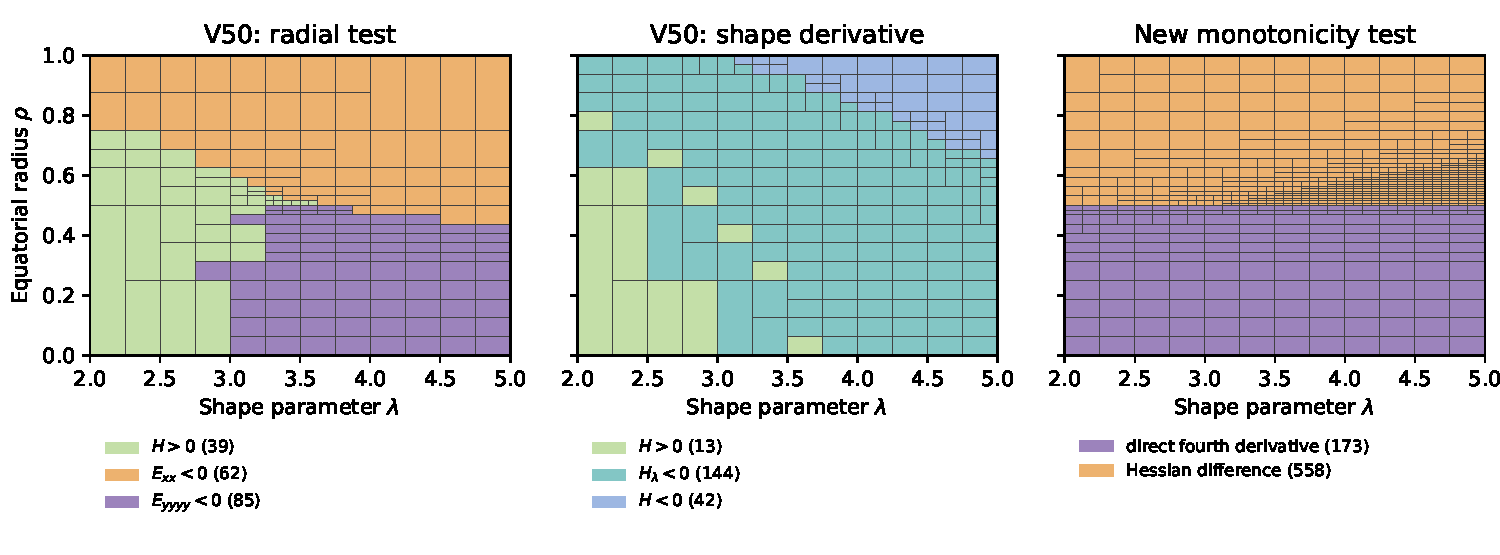
\includegraphics[width=\linewidth]{figures/gate_map.pdf}
\caption{完全に分割された三つの赤道上の検査における実際の終端長方形であり、凡例の数は終端の箱の個数である。最初の二つのパネルは、元の動径方向および形状方向の分割を再現する。三つ目は、ただ一つの符号についての新しい検査である。そこでの色の違いは、同じ四階導関数の二つの表示式を表す。}\label{fig:gate-map}
\end{figure}

\paragraph{記録された区間計算の結果。}
$[2,5]$上の幅$1/4$の十二個の形状スラブから出発した。新しい表には、直接の四階導関数の表示式に対する173個の終端の箱と、Hessianの差に対する558個の終端の箱が含まれる。半径の上端が$s$で半径の下端が正である外側の箱に対して、$H$の区間下界を$a$、$E_{xx}$の上界を$d$とする。$d<a$のとき、有理数$3(d-a)/s^2$は、その箱全体で$E_{yyyy}$の上界である。両方の種類の葉にわたる有理数の上端の最大値は次のとおりであった：
\[
             -109964349/2^{36} < -0.0016 .
\]
整数検査プログラムは、元の葉が出発時の各スラブを被覆することを検証する。第二の実装は、内側の箱では固定曲面エネルギーのTaylor係数を、外側の箱では弦方向における二つのHessian成分の差を積分する。これは元の箱の端点とモードを読み込む。全731個の箱において、局所的な細分の後、1,043個の小片上の上端の最大値は$-1/512$を下回った。したがって、どちらの実装からも上に示した上界が従う。補足ノートは、係数の公式、演算、および両方の被覆検査を与える。同じ元の検査を$1\leq\lambda\leq2$に拡張すると、176個の終端の箱（直接137個、弦39個）が得られ、上界は$-95257877/2^{36}$である。第二の評価プログラムもこれら176個の長方形を被覆し、399個の小片で、上端の最大値は$-0.00031$を下回った。この帯については、二つの独立な上界から、C3で用いる狭義の符号が従う。したがってこの帯では、記録された包囲が成り立つならば、C3における正の境界トレースから、赤道全体で$H>0$であることが従う。

\paragraph{記録された包囲が成り立つ場合の帰結。}
各$2\le\lambda\le5$に対して、$h'=\rho E_{yyyy}/3$であるから、関数$h(\rho)=H(\rho,0;\lambda)$は$(0,1)$上で狭義単調減少である。中心への連続性と、外側の端点における一階導関数のトレースへの連続性により、$h(0)>0>h(1)$ならば内部の半径がちょうど一つ得られ、そうでなければ一つも得られず、これは端点での値が零の場合も同様である。これが分類で用いる動径方向の一意性の議論である。縦方向の排除、二つの遷移の符号と位置、および半径の動きに対する$H_\lambda$は、別個の入力である。元の動径方向の実験には186個の葉があり、39個の箱が$H>0$を、62個が$E_{xx}<0$を、85個が$E_{yyyy}<0$を用いた。199個の葉からなる形状方向の被覆は、$H>0$、$H<0$、$H_\lambda<0$をそれぞれ13個、42個、144個の箱で用いた。これらの個数は実行時間のコストを比較するものではない。

図~\ref{fig:gate-map}において$\rho=1/2$のすぐ外側に箱が集中しているのは、表示の切り替えの位置で生じたものである。中心から離れた内部の重なりの上では、どちらの公式も利用できる。ここに示した計算は、$1/2$での固定した切断を用いる。


\subsection{境界と被覆の接続}
$1\le\lambda\le5$に対して、式~\eqref{eq:near_V}と式~\eqref{eq:window_V}の一様な正の下界は、$z\ne0$である境界点を排除する。境界の赤道上では動径方向成分のみが残る。その係数は$h_b$であり、これは$\bP$でのみ消える。次節の大きな扁長の場合の議論は、$\lambda\ge5$に対してすべての境界点を排除する。薄い扁平の場合の議論はC1--C2と$\lambda=1/32$を共有し、三つの扁長側の区間は端点$2$と$5$を共有する。命題~\ref{prop:sphere}と合わせて、これらの重なり合う範囲は、C1--C6から表~\ref{tab:classification}のすべての行を確立する。

\section{扁長側の裾：明示的な有限包囲への帰着}
\label{sec:prolate-tail}

本節では、計算主張~\ref{comp:c5}および~\ref{comp:c6}の
有理数による包囲の言明を条件として、すべての有限な$\lambda\geq 5$に対する
分類を証明する。
軸上の議論に必要な極での評価を含む解析的な帰着は、
以下で与える。これらの計算主張は、指定されたコンパクトな箱の上の
指定された積分に関するものであり、
停留集合そのものについての言明ではない。

\subsection{正規化と角度係数}
\label{subsec:pt-normalization}

固定した$\lambda\geq 5$に対し、次のようにおく。
\[
 L=\operatorname{diag}(1,1,\lambda),\qquad
 q=(\rho,0,z),\qquad \rho\geq 0,\quad \rho^2+z^2<1,
 \qquad \langle a\rangle_\xi=\frac{1}{4\pi}\int_{S^2}a(\xi)\,d\Omega_\xi .
\]
$LB$から体積保存楕円体への正の相似変換は、
角度エネルギーを変えない。本節では
$E(q)$は参照座標での関数
$\widehat E_\lambda(q)$の略記である。特に、以下の微分はすべて
$q$に関してとる。
$\xi\in S^2$に対し、次のようにおく。
\begin{equation}
\begin{aligned}
 B&=|L^{-T}\xi|^2,&
 D&=|L(\xi-q)|,&
 k&=1-q\cdot\xi,\\
 n&=\frac{L^{-T}\xi}{\sqrt B},&
 \widehat v&=\frac{L(\xi-q)}{D},&
 \gamma&=n\cdot\widehat v=\frac{k}{D\sqrt B}.
\end{aligned}
\label{eq:pt-basic-variables}
\end{equation}
したがって内部では$0<\gamma\leq 1$であり、次が成り立つ。
\[
 E(q)=\langle k\,\arccos^2\gamma\rangle_\xi.
\]
次のように定める。
\begin{equation}
 F(g)=\frac{\pi^2}{4}-\arccos^2g,\qquad
 P(g)=F'(g),\qquad Q(g)=2P(g)+gP'(g).
\label{eq:pt-coefficients}
\end{equation}
$g=1$での値は連続拡張によるものとする。

\begin{lemma}[角度に関する評価]
\label{lem:pt-angular-bounds}
$0\leq g\leq 1$に対し、$A=1+t^2$、$b=1-t^2$として、次が成り立つ。
\begin{align}
 P(g)&=4\int_0^1\frac{dt}{A+bg},&
 Q(g)&=4\int_0^1\frac{2A+bg}{(A+bg)^2}\,dt.
 \label{eq:pt-angular-integrals}
\end{align}
$P$と$Q$はともに正であり、$Q$は非増加で、
$gQ(g)$は非減少である。さらに、次が成り立つ。
\begin{equation}
 gP(g)\leq 2,\qquad
 \pi g-g^2\leq F(g)\leq\pi g,\qquad
 \pi-2g\leq P(g)\leq\pi.
\label{eq:pt-elementary-angular-bounds}
\end{equation}
\end{lemma}

\begin{proof}
表示
$P(g)=2\int_0^\infty(\cosh t+g)^{-1}\,dt$は、
$P(g)=2\arccos(g)/\sqrt{1-g^2}$から従う。
置換$r=\tanh(t/2)$により
式~\eqref{eq:pt-angular-integrals}の第一の積分が得られ、これを微分すると第二の積分が得られる。
被積分関数は$0\leq g\leq1$で一様に正則である。
直接微分すると次を得る。
\[
 Q'(g)=-4\int_0^1\frac{b(3A+bg)}{(A+bg)^3}\,dt\leq0,
 \qquad
 \frac{d}{dg}\{gQ(g)\}
 =8\int_0^1\frac{A^2}{(A+bg)^3}\,dt>0 .
\]
$g=\cos\alpha$と書くと
$gP(g)=2\alpha\cot\alpha\leq2$を得る。
また$P(0)=\pi$であり、次が成り立つ。
\[
 -2\leq P'(g)
 =-2\int_0^\infty\frac{dt}{(\cosh t+g)^2}\leq0.
\]
したがって$\pi-2g\leq P(g)\leq\pi$である。
$F(0)=0$を用いて$0$から積分すると、$F$に対する主張の評価が
得られる。
\end{proof}

これらの係数は、$g=1$の近くで$\arccos$を評価することなく
包囲することもできる。
$h=(1-g)/2\in[0,1/2]$に対し、次のようにおく。
\begin{equation}
 a_0=1,\qquad
 a_{n+1}=a_n\frac{2n+2}{2n+3},\qquad
 q_n=(4+2n)a_n-(n+1)a_{n+1}>0 .
\label{eq:pt-positive-series-coefficients}
\end{equation}
式~\eqref{eq:pt-angular-integrals}の第一の積分を
一様収束する等比級数に展開すると、次がわかる。
\begin{equation}
 P(g)=2\sum_{n\geq0}a_nh^n,\qquad
 Q(g)=\sum_{n\geq0}q_nh^n .
\label{eq:pt-positive-series}
\end{equation}
実際$a_n=\int_0^1(1-t^2)^n\,dt$であり、これから漸化式が得られ、
また
$q_n=2a_n(n^2+5n+5)/(2n+3)>0$である。
特に、$Q$の級数の打ち切りは下界である。
$a_n\leq1$であるから、次が成り立つ。
\begin{equation}
 2\sum_{n=0}^N a_nh^n
 \leq P(g)
 \leq 2\sum_{n=0}^N a_nh^n+4h^{N+1}.
\label{eq:pt-series-enclosures}
\end{equation}
これらの不等式は、計算主張~\ref{comp:c5}の係数表で用いる
解析的な剰余の上界を定める。

\subsection{横断方向のHessianと弦の恒等式}
\label{subsec:pt-chord}

$\rho>0$に対して$H=E_\rho/\rho$とおき、$\rho=0$へは
$H=E_{yy}$によって拡張する。代表点$(\rho,0,z)$では、
回転対称性により$E_{yy}=E_\rho/\rho$となる。
ここで$y=q_2$は、$L_{22}=1$であるから、
$L$に対する物理的な横断方向の座標でもある。

\begin{lemma}[有界な弦表示]
\label{lem:pt-chord-representation}
内部の$q$に対し、$e\in S^2$をとり、次のように定める。
\begin{equation}
\begin{gathered}
 m=e_z,\quad j=e_y^2,\quad v=q\cdot e,\quad
 \delta=1-|q|^2,\quad d=\sqrt{\delta+v^2},\\
 C=|Le|^2=1+(\lambda^2-1)m^2,\quad
 U=1-C^{-1},\quad \ell_\sigma=d-\sigma v,\\
 \xi_\sigma=q+\sigma\ell_\sigma e,\qquad
 B_\sigma=|L^{-T}\xi_\sigma|^2,\\
 w_\sigma=\frac{1-\sigma v/d}{2},\qquad
 \gamma_\sigma=\frac{d}{\sqrt{CB_\sigma}},
 \qquad \sigma\in\{-1,1\}.
\end{gathered}
\label{eq:pt-chord-variables}
\end{equation}
このとき$w_\sigma\geq0$、$w_++w_-=1$であり、次が成り立つ。
\begin{equation}
 H=\left\langle
 \sum_{\sigma=\pm1}w_\sigma
 \left[
 \frac{d^2(1-j/C)}{C^{3/2}}\,
 \frac{P(\gamma_\sigma)}{\sqrt{B_\sigma}}
 -
 \frac{j(dU-\sigma v)^2}{\sqrt C}\,
 \frac{Q(\gamma_\sigma)}{\sqrt{B_\sigma}}
 \right]\right\rangle_e .
\label{eq:pt-chord-hessian}
\end{equation}
重み付きの負の因子は、次の厳密な恒等式を満たす。
\begin{equation}
 \sum_{\sigma=\pm1}w_\sigma(dU-\sigma v)^2
 =\delta U^2+(1+U)^2v^2.
\label{eq:pt-paired-negative-identity}
\end{equation}
\end{lemma}

\begin{proof}
$q$に依存する変数変換を行う前に、
まず元の球面上で微分する。
$b_y=n_y-\gamma\widehat v_y$とおく。
$\xi$を固定すると、次が成り立つ。
\[
 D_y=-\widehat v_y,\qquad
 \gamma_y=-b_y/D,\qquad
 (\widehat v_y)_y=-(1-\widehat v_y^2)/D,\qquad
 (b_y)_y=\{b_y\widehat v_y+
 \gamma(1-\widehat v_y^2)\}/D.
\]
また$k=D\sqrt B\,\gamma$および$k_y=-\sqrt B\,n_y$である。
したがって$k\arccos^2\gamma$を二回微分すると次を得る。
\begin{equation}
 H=\left\langle\frac{\sqrt B}{D}
 \left[
 P(\gamma)\gamma^2(1-\widehat v_y^2)
 -Q(\gamma)(n_y-\gamma\widehat v_y)^2
 \right]\right\rangle_\xi .
\label{eq:pt-original-transverse-hessian}
\end{equation}
これらの微分は、開球の各コンパクト部分集合上で正当であり、
そこでは$D$は正の下界をもつ。

直線$q+\mathbb R e$と球面との交点は、
ちょうど式~\eqref{eq:pt-chord-variables}の$\xi_\sigma$である。
$\xi_\sigma\cdot(\sigma e)=d$であるから、
$q$からの動径射影により次を得る。
\[
 d\Omega_\xi=\frac{\ell_\sigma^2}{d}\,d\Omega_e .
\]
両方の符号と方向の全球面を用いると、各曲面上の点が
二回覆われる。したがって変換後の積分には因子
$1/2$が付く。
二つの端点では、次が成り立つ。
\[
 k_\sigma=\ell_\sigma d,\quad
 D_\sigma=\ell_\sigma\sqrt C,\quad
 \widehat v_{y,\sigma}=\frac{\sigma e_y}{\sqrt C},\quad
 n_{y,\sigma}-\gamma_\sigma\widehat v_{y,\sigma}
 =\frac{\sigma e_y}{\sqrt{B_\sigma}}\,(dU-\sigma v).
\]
式~\eqref{eq:pt-original-transverse-hessian}に代入すると、
$w_\sigma=\ell_\sigma/(2d)$として式~\eqref{eq:pt-chord-hessian}が
得られる。
最後に$\sum_\sigma\sigma w_\sigma=-v/d$および
$d^2=\delta+v^2$であるから、
式~\eqref{eq:pt-paired-negative-identity}の左辺は
$d^2U^2+2Uv^2+v^2$である。
\end{proof}

固定した有限の$\lambda$に対し、この公式は$q$が
閉球に近づくとき有界である。実際、
$B_\sigma\geq\lambda^{-2}$、$|v|\leq d$であり、
式~\eqref{eq:pt-chord-hessian}の角括弧の中の式は
$d=0$で$O_\lambda(d^2)$である。そこでの値は零とおくことができる。
したがって、つぶれる弦の端点での特異な距離は、
射影のJacobianによってすでに相殺されている。この
相殺は、動くJacobianの微分を
伴わない。

\subsection{三つの一次元係数}
\label{subsec:pt-three-coefficients}

$l=\sqrt{\lambda^2-1}$とする。$x\in[0,l]$に対し、次のようにおく。
\[
\begin{aligned}
 m&=x/l,& C&=1+x^2,& U&=1-C^{-1},\\
 Y&=\frac{1-m^2}{2},& J_2&=\frac{(1-m^2)^2}{8},&
 Q_C&=Q(C^{-1/2}).
\end{aligned}
\]
ここでの記号$J_2$は方位角モーメントを表し、
一階微分の核$gP(g)-\arccos^2g$ではない。
$P_i(l)$と$N_i(l)$を、次の密度を
$0\leq x\leq l$上で積分することによって定める。
\begin{equation}
\begin{array}{c|c|c}
 i & \text{density of }P_i & \text{density of }N_i\\ \hline
 c & 2(1-Y/C)/C
   & Q_C U^2Y/\sqrt C\\[2pt]
 e & \{1+Y-(Y+J_2)/C\}/C
   & Q_C(1+U)^2J_2/\sqrt C\\[2pt]
 p & (1+m^2)(1-Y/C)/C
   & Q_C(1+U)^2m^2Y/\sqrt C .
\end{array}
\label{eq:pt-three-coefficient-densities}
\end{equation}

\begin{lemma}[凸結合による評価]
\label{lem:pt-convex-bound}
内部のすべての$q=(\rho,0,z)$に対し、次が成り立つ。
\begin{equation}
 lH(q;\lambda)\leq
 \delta\{P_c(l)-N_c(l)\}
 +\rho^2\{P_e(l)-N_e(l)\}
 +z^2\{P_p(l)-N_p(l)\},
 \qquad \delta+\rho^2+z^2=1.
\label{eq:pt-convex-bound}
\end{equation}
さらに、
\begin{equation}
 P_c(l)\leq\frac{3\pi}{4},\qquad
 P_e(l)\leq\frac{3\pi}{4},\qquad
 P_p(l)\leq\frac{\pi}{2},
\label{eq:pt-positive-coefficient-bounds}
\end{equation}
が成り立ち、各$N_i(l)$は$l>0$で非減少である。
\end{lemma}

\begin{proof}
$y=d/\sqrt C$、$a=\sqrt{B_\sigma}\leq1$とおく。
このとき$\gamma_\sigma=y/a\geq y$である。
$gQ(g)$の単調性と$Q$の減少性により次を得る。
\[
 \frac{Q(\gamma_\sigma)}{\sqrt{B_\sigma}}
 \geq Q(d/\sqrt C)\geq Q(C^{-1/2})=Q_C.
\]
$d=0$の場合は、いま述べた有界な拡張から従う。
式~\eqref{eq:pt-chord-hessian}の正の部分については、
$gP(g)\leq2$と$2d\leq1+d^2$により次を得る。
\[
 \sum_\sigma w_\sigma
 \frac{d^2(1-j/C)}{C^{3/2}}
 \frac{P(\gamma_\sigma)}{\sqrt{B_\sigma}}
 \leq \frac{(1+\delta+v^2)(1-j/C)}{C}.
\]
負の部分については、評価する前に、
対の恒等式~\eqref{eq:pt-paired-negative-identity}を用いる。

$m=e_z$を固定すると、方位角平均は次を満たす。
\[
 \overline j=Y,\qquad
 \overline{v^2}=\rho^2Y+z^2m^2,\qquad
 \overline{jv^2}=\rho^2J_2+z^2m^2Y.
\]
この平均の後、被積分関数は$m$について偶であるから、正規化した
球面平均は$m\in[0,1]$上の積分になる。
$1=\delta+\rho^2+z^2$を用いて、正の部分を
式~\eqref{eq:pt-three-coefficient-densities}の三つの係数にまとめる。
すると置換$x=lm$により式~\eqref{eq:pt-convex-bound}が示される。

直接積分すると次を得る。
\[
 P_c(l)=\left(\frac32+\frac{1}{2l^2}\right)\arctan l
 -\frac{1}{2l}\leq\frac32\arctan l\leq\frac{3\pi}{4}.
\]
$P_e$の密度の非負の項を落とすと
$P_e\leq(3/2)\arctan l$を得る。
同様に次が成り立つ。
\[
 P_p(l)\leq\arctan l+\frac{l-\arctan l}{l^2}
 \leq\arctan l+\arctan(1/l)=\frac{\pi}{2}.
\]
ここで
$(l-\arctan l)/l^2\leq l/(1+l^2)\leq\arctan(1/l)$であり、
これは$\arctan r\geq r/(1+r^2)$から従う。

$N_c$と$N_e$については、$x$を固定する。$l$が増加すると、
$Y$と$J_2$はともに既存の定義域上で増加し、
定義域$[0,l]$は広がる。残りの因子はすべて非負で、
$l$に依存しない。
$N_p$については、代わりに$m\in[0,1]$に戻る。
\[
 N_p(l)=\int_0^1
 \frac{l}{\sqrt C}\,Q(C^{-1/2})(1+U)^2m^2Y\,dm .
\]
$m$を固定すると、因子$l/\sqrt C$、
$Q(C^{-1/2})$、$(1+U)^2$はすべて$l$について非減少である。
これで主張した単調性が示された。
\end{proof}

次のようにおく。
\[
 \overline P_c=\overline P_e=3\pi/4,\qquad
 \overline P_p=\pi/2.
\]
計算主張~\ref{comp:c5}の一次元の部分は、
次の包囲不等式の有限個の一覧である。
\begin{equation}
\begin{array}{c|ccc}
 \lambda_0,\ l_0=\sqrt{\lambda_0^2-1}
 &\overline P_c-N_c(l_0)
 &\overline P_e-N_e(l_0)
 &\overline P_p-N_p(l_0)\\ \hline
 8 &<-1/20&<-2/5&<-3/5\\
 5 &<1&<1&<-3/16 .
\end{array}
\label{eq:pt-anchor-assertions}
\end{equation}
これらは式~\eqref{eq:pt-three-coefficient-densities}の
積分の包囲であり、いくつかの空間点での
$H$の評価ではない。
そのために用いる有限和は明示的に指定できる。
$N=2048$、$m_j=j/N$、$C_j=1+l^2m_j^2$、
$U_j=1-C_j^{-1}$、$T_j=1-m_{j+1}^2$とし、次のようにおく。
\[
 Q_{12}(g)=\sum_{n=0}^{12}q_n\{(1-g)/2\}^n,\qquad
 \omega_j=\frac{l}{N}\,
             \frac{Q_{12}(C_j^{-1/2})}{\sqrt{C_{j+1}}}.
\]
$[m_j,m_{j+1}]$上での非負の因子の単調性により、
次の下方和を得る。
\begin{equation}
\begin{split}
 N_c(l)&\geq\sum_{j=0}^{N-1}
                \omega_j U_j^2T_j/2,\\
 N_e(l)&\geq\sum_{j=0}^{N-1}
                \omega_j(1+U_j)^2T_j^2/8,\\
 N_p(l)&\geq\sum_{j=0}^{N-1}
                \omega_j(1+U_j)^2m_j^2T_j/2 .
\end{split}
\label{eq:pt-explicit-anchor-darboux}
\end{equation}
たとえば、$Q(C^{-1/2})$と$U$は$m$とともに増加し、
一方$1/\sqrt C$と$1-m^2$は減少する。
$Q$の級数の正の尾は捨ててよい。
記録された生成プログラムは、これらの和を$l=\sqrt{24}$と
$l=\sqrt{63}$において、$96$ビットの外向き丸めのArb演算で包囲する。
この有限の演算と、その出力である厳密な有理数の界は、
計算主張~\ref{comp:c5}の一部である。

\begin{lemma}[非有界領域と極領域]
\label{lem:pt-unbounded-and-polar}
アンカー不等式~\eqref{eq:pt-anchor-assertions}を仮定すると、次が成り立つ。
\begin{align}
 lH&<-1/20
 &&(\lambda\geq8,\ |q|<1),\label{eq:pt-unbounded-bound}\\
 lH&<-7/50
 &&(\lambda\geq5,\ |q|<1,\ 1-z^2\leq\lambda^{-2}).
 \label{eq:pt-polar-horizontal-bound}
\end{align}
\end{lemma}

\begin{proof}
$N_i$の単調性と式~\eqref{eq:pt-positive-coefficient-bounds}により、
式~\eqref{eq:pt-anchor-assertions}の各行は、より大きなすべての
$\lambda$に伝わる。第一行と
式~\eqref{eq:pt-convex-bound}の非負の重みから式~\eqref{eq:pt-unbounded-bound}が得られる。
第二行については、$S=\sqrt{1-z^2}$とおく。
$\delta+\rho^2=S^2$であるから、これにより次を得る。
\[
 lH<S^2-\frac{3}{16}z^2
 =\frac{19}{16}S^2-\frac{3}{16}.
\]
$S\leq1/\lambda$かつ$\lambda\geq5$ならば、これは高々
$19/400-75/400=-7/50$である。
\end{proof}

\subsection{5と8の間の有限の橋}
\label{subsec:pt-finite-bridge}

残るのは、次のコンパクト領域上で$H$を評価することである。
\begin{equation}
 \mathcal D_{\rm br}=
 \left\{(\lambda,\rho,z):
 5\leq\lambda\leq8,\quad \rho,z\geq0,\quad
 \rho^2+z^2\leq1,\quad 1-z^2\geq\lambda^{-2}\right\}.
\label{eq:pt-bridge-domain}
\end{equation}
下半分は$z$に関する鏡映から得られる。
計算主張~\ref{comp:c5}の有限の部分は、この領域の分割に関するものであり、
特異な二階微分の被積分関数ではなく
弦の公式を用いる。
包囲の規則を明示的に与える。

$a=\sqrt B>0$および$y=d/\sqrt C$に対し、係数の因子は次のとおりである。
\begin{align}
 \frac{P(y/a)}a
 &=4\int_0^1\frac{dt}{Aa+by},&
 \frac{Q(y/a)}a
 &=4\int_0^1\frac{2Aa+by}{(Aa+by)^2}\,dt.
 \label{eq:pt-scaled-coefficient-integrals}
\end{align}
両方の式は、$a$と$y$のそれぞれについて非増加である。
第二の式については、これは
$(2x+s)/(x+s)^2$を$x>0$と$s\geq0$に関して微分することで従う。
橋の上では$B\geq1/64$かつ$1\leq C\leq64$であるから、これらの
係数の包囲は正の分母をもつ。
幾何学的に実現可能な対$0\leq y\leq a$のみが現れる。
包囲する長方形
$a\in[a_-,a_+]$、$y\in[y_-,y_+]$に対し、有効な選び方には次が含まれる。
\begin{equation}
 \frac{P(y/a)}a
 \leq\frac{P(\min\{1,y_-/a_-\})}{a_-},\qquad
 \frac{Q(y/a)}a
 \geq\frac{Q(\min\{1,y_+/a_+\})}{a_+}.
\label{eq:pt-geometric-coefficient-clipping}
\end{equation}
いずれかの比が高々1であるとき、対応する不等式は
それぞれについての単調性から従う。
$y_->a_-$ならば、$P(y/a)/a\leq2/y_-\leq2/a_-$を用いる。
$y_+>a_+$ならば、$Q(y/a)/a\geq Q(1)/a_+$を用いる。
したがって、係数の引数を1に切り詰めることは、
幾何とこれらの不等式によって正当化される。正係数の
級数は$0\leq g\leq1$に対してのみ用いる。

角度セルと外側のパラメータ箱の上で、次のようにおく。
\[
 p_\sigma\geq
 \frac{P(\gamma_\sigma)}{\sqrt{B_\sigma}},
 \qquad
 n_\sigma\leq
 \frac{Q(\gamma_\sigma)}{\sqrt{B_\sigma}},
 \qquad n_\sigma\geq0.
\]
これらは、式~\eqref{eq:pt-scaled-coefficient-integrals}と
式~\eqref{eq:pt-series-enclosures}における端点での単調性から
得られる。
$p_i\geq p_{-i}$かつ
$n_k\geq n_{-k}$となるように$i$と$k$を選び、$A_\sigma=dU-\sigma v$とおく。
このとき、次のセルごとの不等式で十分である。
\begin{align}
 \sum_\sigma w_\sigma
 \frac{P(\gamma_\sigma)}{\sqrt{B_\sigma}}
 &\leq p_{-i}+\sup(w_i)(p_i-p_{-i}),
 \label{eq:pt-positive-cell-bound}\\
 \sum_\sigma w_\sigma A_\sigma^2
 \frac{Q(\gamma_\sigma)}{\sqrt{B_\sigma}}
 &\geq n_{-k}\{\delta U^2+(1+U)^2v^2\}
 \nonumber\\
 &\quad +(n_k-n_{-k})\inf(w_k)\inf(A_k^2).
 \label{eq:pt-negative-cell-bound}
\end{align}
第一の不等式は$\sum w_\sigma=1$を用いる。
第二の不等式は、厳密な
対の恒等式~\eqref{eq:pt-paired-negative-identity}を用いる。その
追加項の因子はすべて非負である。したがって、大きな負の
寄与は、区間による評価を適用する前に保たれる。

これらの評価に必要な方位角積分は初等的である。
$m\geq0$に対し、
$v=v_0+v_1\cos\phi$と書く。ここで
$v_0=zm$、$v_1=\rho\sqrt{1-m^2}$であり、また
$j=(1-m^2)\sin^2\phi$である。
幅$\Delta$のセル$I=[\alpha,\beta]$に対し、
$\overline f_I=\Delta^{-1}\int_I f(\phi)\,d\phi$とおく。
必要なモーメントは次のとおりである。
\begin{align}
 \overline{\cos\phi}_I
 &=\frac{\sin\beta-\sin\alpha}{\Delta},&
 \overline{\cos^2\phi}_I
 &=\frac12+\frac{\sin2\beta-\sin2\alpha}{4\Delta},
 \label{eq:pt-azimuth-moments-one}\\
 \overline{\sin^2\phi\cos\phi}_I
 &=\frac{\sin^3\beta-\sin^3\alpha}{3\Delta},&
 \overline{\sin^2\phi\cos^2\phi}_I
 &=\frac18-\frac{\sin4\beta-\sin4\alpha}{32\Delta}.
 \label{eq:pt-azimuth-moments-two}
\end{align}
特に、次が成り立つ。
\begin{align}
 \overline{v^2}_I
 &=(v_0+v_1\overline{\cos\phi}_I)^2
 +v_1^2\{\overline{\cos^2\phi}_I-
             \overline{\cos\phi}_I^{\,2}\},\nonumber\\
 \overline{jv^2}_I
 &=(1-m^2)\left[
 v_0^2\overline{\sin^2\phi}_I
 +2v_0v_1\overline{\sin^2\phi\cos\phi}_I
 +v_1^2\overline{\sin^2\phi\cos^2\phi}_I\right],\nonumber\\
 \overline{d^2(1-j/C)}_I
 &=\delta+\overline{v^2}_I
 -\frac{\delta\overline j_I+\overline{jv^2}_I}{C}.
 \label{eq:pt-azimuth-moment-combinations}
\end{align}
負の項に対する
$\delta U^2\overline j_I+(1+U)^2\overline{jv^2}_I$と
合わせて、これらの公式は、
式~\eqref{eq:pt-chord-hessian}への各角度セルの寄与の明示的な上側の包囲を
与える。
すべてのモーメントは、その端点で外向きに包囲される。
残る$m$についての積分は、正の正規化された重みをもつ
セル上の値域によって包囲される。符号の主張を行う前に、幾何は
$\mathcal D_{\rm br}$と交わらせる。

計算主張~\ref{comp:c5}に記録された有限の包囲の言明は、
次のとおりである。
\begin{equation}
\begin{array}{c|r|r|c}
 \lambda\text{-slab}&
 \text{nonempty negative leaves}&
 \text{empty leaves}&
 \text{uniform upper bound for }H\\ \hline
 {[5,6]}&1539&3&-68778309/68719476736\\
 {[6,7]}&266&2&-9210649/8589934592\\
 {[7,8]}&119&0&-1095717/1073741824 .
\end{array}
\label{eq:pt-bridge-enclosure-table}
\end{equation}
細分では、上端点が$-1/1000$を超えていた元の親が、それぞれ72個、5個、2個置き換えられる。元の核は二進分割による両方の子の上で評価する。形状の区間とそれらが共有する端点は変わらない。各行は、
式~\eqref{eq:pt-bridge-domain}との指定された共通部分の完全な被覆と、
すべての空でない葉に対する表示された包囲の両方を主張する。したがってこれは有限で
検証可能な全称命題であり、葉の厳密な端点、
親子関係および有理数の界は
計算付録で与えられる。負の上界は、
葉の体積の和だけから導かれるものではない。

\begin{proposition}[一様な横断方向の負値性]
\label{prop:pt-horizontal-negative}
計算主張~\ref{comp:c5}のもとで、次が成り立つ。
\begin{equation}
 \sqrt{\lambda^2-1}\,H(q;\lambda)<-1/250
 \qquad(\lambda\geq5,\ |q|<1).
\label{eq:pt-global-horizontal}
\end{equation}
\end{proposition}

\begin{proof}
補題~\ref{lem:pt-unbounded-and-polar}の領域と
式~\eqref{eq:pt-bridge-domain}の領域が、すべての場合を覆う。
式~\eqref{eq:pt-bridge-enclosure-table}の上界はすべて
$-1/1000$より小さい。
橋の上では$\sqrt{\lambda^2-1}\geq\sqrt{24}>4$であるから、
これによりそこでは式~\eqref{eq:pt-global-horizontal}が得られる。
他の二つの界$-1/20$と$-7/50$は、
$-1/250$より小さい。
\end{proof}

\subsection{軸に対する明示的な極冠の入力}
\label{subsec:pt-polar-cap}

命題~\ref{prop:pt-horizontal-negative}は、極の近くの点も含め、
$\rho>0$であるすべての点をすでに扱っている。
残る軸上での証明には、薄い冠における軸方向の評価が
追加で必要である。その積分の入力をここで導く。
次のようにおく。
\[
 \epsilon=\lambda^{-1},\quad
 \mu=\xi_z,\quad s=\sqrt{1-\mu^2},\quad
 S=\sqrt{1-z^2},\quad
 \xi=(s\cos\phi,s\sin\phi,\mu),
\]
そして次のように定める。
\begin{equation}
\begin{aligned}
 A_0&=s^2+\rho^2-2\rho s\cos\phi,&
 d_0^2&=(\mu-z)^2+\epsilon^2A_0,\\
 B&=s^2+\epsilon^2\mu^2,&
 k&=1-z\mu-\rho s\cos\phi,&
 \gamma&=\frac{\epsilon k}{d_0\sqrt B}.
\end{aligned}
\label{eq:pt-cap-variables}
\end{equation}
ここでの記号$d_0,A_0$は冠の座標に関するものであり、
弦の変数$d,A_\sigma$とは別のものである。

$\langle k\rangle_\xi=1$であるから、
$E=\pi^2/4-\langle kF(\gamma)\rangle_\xi$を微分すると次を得る。
\begin{equation}
 E_z=\frac{1}{4\pi}\int_0^{2\pi}\int_{-1}^1 I\,d\mu\,d\phi,
 \quad
 I=\mu(F+\gamma P)
       -\frac{k\gamma P(\mu-z)}{d_0^2}.
\label{eq:pt-cap-first-derivative}
\end{equation}
たとえば、
$\gamma_z/\gamma=-\mu/k+(\mu-z)/d_0^2$によってこの公式を
直接確かめられる。

北側の冠全体を次のようにパラメータ表示する。
\begin{equation}
 0<\epsilon\leq\frac15,\quad 0\leq w,u\leq1,\qquad
 z=\sqrt{1-\epsilon^2w^2},\qquad
 \rho=\epsilon wu.
\label{eq:pt-cap-parameterization}
\end{equation}
このとき$S=\epsilon w$、$\rho\leq S$および
$z\geq\sqrt{24/25}>3/4$である。
$c=3/4$、$\eta=1/64$とおく。
式~\eqref{eq:pt-cap-first-derivative}のうち
$c\leq\mu\leq z$の部分は非負である。
残る北側の帯$\mu>z$については、第一項は
非負であり、一方で次が成り立つ。
\[
 \frac{k\gamma P(\mu-z)}{d_0^2}
 =\frac{\sqrt B}{\epsilon}\,
   \gamma^2P\,\frac{\mu-z}{d_0}
 \leq \frac{2\sqrt B}{\epsilon}
 \leq2\sqrt{1+w^2}.
\]
したがって、その$E_z$への正規化された寄与は少なくとも
$-\epsilon^2w^2\sqrt{1+w^2}/(1+z)$である。

南側の帯$\theta=\arccos\mu\in[\pi-\eta,\pi]$については、
式~\eqref{eq:pt-cap-first-derivative}の第二項は
非負であり、落としてよい。
式~\eqref{eq:pt-elementary-angular-bounds}により、
$F+\gamma P\leq2\pi\gamma$である。
$d_0\geq z-\mu$、$\sqrt B\geq s$を用い、最後の評価を行う前に
$\phi$について平均する。
$k$の平均は$1-z\mu$であり、
$\mu<0$に対して$(1-z\mu)/(z-\mu)\leq1/z$である。
したがって、南側の帯の$E_z$への寄与は少なくとも
$-\pi\epsilon\eta/z$である。

保持した長方形
\[
 \theta\in[\arccos(3/4),\,\pi-1/64],\qquad
 \phi\in[0,\pi],
\]
の上で、次のようにおく。
\[
 T_0=\frac{s}{\sqrt B},\qquad
 f_1=\mu k,\qquad
 f_2=\mu k+\frac{k^2(z-\mu)}{d_0^2}.
\]
このとき次が成り立つ。
\[
 \frac{Is}{\epsilon}
 =\frac{T_0}{d_0}
       \left[f_1\frac{F(\gamma)}{\gamma}+f_2P(\gamma)\right].
\]
$\gamma=0$では、商$F(\gamma)/\gamma$を
$\pi$と定める。各係数の符号を保ったまま
両側からの角度評価を適用すると、次を得る。
\begin{equation}
 \mathcal L(\theta,\phi;\epsilon,w,u)=
 \frac{T_0}{d_0}
 \left\{\pi(f_1+f_2)
        -\gamma\bigl[(f_1)_++2(f_2)_+\bigr]\right\}
 \leq\frac{Is}{\epsilon},
 \quad x_+=\max(x,0).
\label{eq:pt-cap-lower-envelope}
\end{equation}
したがって、$\phi$に関する鏡映を用いると、次が成り立つ。
\begin{equation}
\begin{split}
 \lambda E_z\geq \mathcal B(\epsilon,w,u)
 :={}&\frac{1}{2\pi}
 \int_0^\pi
 \int_{\arccos(3/4)}^{\pi-1/64}
       \mathcal L(\theta,\phi;\epsilon,w,u)\,d\theta\,d\phi\\
 &-\frac{\pi}{64z}
 -\frac{\epsilon w^2\sqrt{1+w^2}}{1+z}.
\end{split}
\label{eq:pt-cap-computational-integral}
\end{equation}
この保持した長方形の上には小さな分母は現れない。すなわち、
$d_0\geq z-\mu\geq\sqrt{24/25}-3/4>0$および
$s\geq\sin(1/64)>0$である。
したがって右辺は$\epsilon=0$でも連続である。
この端点は下界の積分のコンパクト化にすぎず、
$\lambda=\infty$でのエネルギーを定義しているわけではない。

計算主張~\ref{comp:c6}の正確な言明は次のとおりである。
\begin{equation}
\begin{gathered}
 \mathcal B(\epsilon,w,u)\geq
 r_{\rm cap}:=
 \frac{47473218194072764542240096942353646083}{2^{127}}
 >\frac14,\\
 \left(0\leq\epsilon\leq\frac15,\ 0\leq w,u\leq1\right).
\end{gathered}
\label{eq:pt-cap-computational-assertion}
\end{equation}
明確にするために述べると、その記録された有限分割は
$16\times8\times8=1,024$個の外側の箱である。
\[
 \epsilon\in[i/80,(i+1)/80],\qquad
 w\in[j/8,(j+1)/8],\qquad
 u\in[k/8,(k+1)/8].
\]
保持した$\theta$の区間は$96$個の等しい
セルに分割し、$[0,\pi]$は$48$個の等しい$\phi$のセルに分割する。
各セル上で式~\eqref{eq:pt-cap-lower-envelope}の値域を
$128$ビットの外向き丸めのArb演算で包囲し、
正のセル面積を掛ける。
式~\eqref{eq:pt-cap-computational-integral}で
引かれる二つの項は、
必要な上向きの方向に評価する。
これは各外側の箱の全体にわたる下方Darboux包囲であり、
経験的な誤差評価を伴う求積値ではない。

第二の実装は、元の各外側の箱の上で、144ビットで$120\times64$個の角度セルを用いる。その最小の下端点は、$2^{-48}$の倍数に切り下げると、$107156256170842/2^{48}>r_{\rm cap}$である。どちらの計算も同じ解析的な下側包絡を積分する。

\begin{lemma}[北側の冠での評価]
\label{lem:pt-north-cap}
計算主張~\ref{comp:c6}のもとで、
$\lambda\geq5$、$z>0$、$1-z^2\leq\lambda^{-2}$を満たすすべての内部の点に対し、次が成り立つ。
\begin{equation}
 E_z(\rho,z;\lambda)\geq\frac{1}{4\lambda}.
\label{eq:pt-north-cap}
\end{equation}
\end{lemma}

\begin{proof}
そのような点はすべて式~\eqref{eq:pt-cap-parameterization}の形をしている。
式~\eqref{eq:pt-cap-computational-integral}と
式~\eqref{eq:pt-cap-computational-assertion}を組み合わせればよい。
\end{proof}

\subsection{軸上での符号付き角による証明}
\label{subsec:pt-axis}

\begin{lemma}[軸上での一様な正値性]
\label{lem:pt-axis-positive}
計算主張~\ref{comp:c6}のもとで、次が成り立つ。
\begin{equation}
 \frac{E_z(0,z;\lambda)}{z}
 \geq\frac{3}{10\lambda^2}>0
 \qquad(\lambda\geq5,\ 0<|z|<1).
\label{eq:pt-axis-positive}
\end{equation}
この商は$z=0$で連続な値$E_{zz}(0,0;\lambda)$をもち、
そこでも同じ下界が成り立つ。
\end{lemma}

\begin{proof}
$\epsilon=1/\lambda$、$s=\sqrt{1-\mu^2}$、
$B=s^2+\epsilon^2\mu^2$および
$D_2=(\mu-z)^2+\epsilon^2s^2$とおく。
$-1<\mu<1$に対し、子午面内の二つの
ベクトルの間の符号付き角は次のとおりである。
\begin{equation}
 a(\mu,z)=
 \arctan\frac{\mu-z}{\epsilon s}
 -\arctan\frac{\epsilon\mu}{s}.
\label{eq:pt-signed-meridional-angle}
\end{equation}
どちらのベクトルも水平成分が正である。
内部の基点に対してはそれらの内積は正であるから、
$|a|<\pi/2$かつ$a^2=\arccos^2\gamma$である。
したがって次が成り立つ。
\begin{equation}
 E(0,z)=\frac12\int_{-1}^1(1-z\mu)a(\mu,z)^2\,d\mu.
\label{eq:pt-axis-energy}
\end{equation}

$k=1-z\mu$として、直接微分すると次を得る。
\begin{equation}
 a_z=-\frac{\epsilon s}{D_2},\qquad
 a_\mu=\frac{\epsilon k}{sD_2}-\frac{\epsilon}{sB},
 \qquad
 ka_z+s^2a_\mu=-\frac{\epsilon s}{B}.
\label{eq:pt-axis-transport-identity}
\end{equation}
この最後の恒等式を
式~\eqref{eq:pt-axis-energy}の微分に用い、
$-s^2\partial_\mu(a^2)$を部分積分すると、次を得る。
\begin{equation}
 E_z=\frac12\int_{-1}^1
       \left[-3\mu a^2-\frac{2\epsilon s}{B}a\right]\,d\mu .
\label{eq:pt-axis-integrated-derivative}
\end{equation}
固定した$\epsilon>0$と$|z|<1$に対し、$D_2$と$B$は
$[-1,1]$上で正の下界をもつ。
現れうる因子$1/s$は可積分であり、
$s^2a^2$は両端点で零に収束する。
したがって、微分と部分積分は、
まず端点を切り落とし、その後に極限をとることで正当化される。

鏡映により$z>0$としてよい。
$0<\mu<1$に対し、次のように定める。
\[
 b=\arctan\frac{\epsilon\mu}{s},\qquad
 \theta_\pm=\arctan\frac{\mu\pm z}{\epsilon s},\qquad
 D_a=\theta_+-\theta_-,\qquad
 \Sigma=\theta_++\theta_--2b .
\]
$a(\mu,z)=\theta_--b$および
$a(-\mu,z)=-(\theta_+-b)$であるから、
式~\eqref{eq:pt-axis-integrated-derivative}で$\mu$と$-\mu$を対にすると、次の因数分解を得る。
\begin{equation}
\begin{aligned}
 \frac{E_z}{z}
 &=\frac12\int_0^1\frac{D_a}{z}
          \left(3\mu\Sigma+\frac{2\epsilon s}{B}\right)\,d\mu,\\
 \frac{D_a}{z}
 &=\int_{-1}^1
   \frac{\epsilon s\,dt}{(\mu+tz)^2+\epsilon^2s^2}.
\end{aligned}
\label{eq:pt-axis-reflected-factorization}
\end{equation}

$L_\pm=(\mu\pm z)^2+\epsilon^2s^2$および
$S=\sqrt{1-z^2}$とおく。
正弦と余弦の加法公式により次を得る。
\begin{equation}
 \sin\Sigma=
 \frac{2\epsilon\mu s(S^2-\epsilon^2)}
      {B\sqrt{L_+L_-}}.
\label{eq:pt-axis-angle-sum-sign}
\end{equation}
完全を期して記すと、
\[
\begin{aligned}
 \sin(\theta_++\theta_-)
 &=\frac{2\epsilon s\mu}{\sqrt{L_+L_-}},\\
 \cos(\theta_++\theta_-)
 &=\frac{\epsilon^2s^2-\mu^2+z^2}{\sqrt{L_+L_-}}.
\end{aligned}
\]
であり、また
$\sin(2b)=2\epsilon\mu s/B$、
$\cos(2b)=(s^2-\epsilon^2\mu^2)/B$である。
これらを代入すると、分子は$S^2-\epsilon^2$に帰着する。
また$\theta_++\theta_-\in[0,\pi)$かつ$2b\in[0,\pi)$であるから、
$\Sigma\in(-\pi,\pi)$である。
したがって$S\geq\epsilon$ならば$\Sigma\geq0$である。

その場合、式~\eqref{eq:pt-axis-reflected-factorization}で
$\mu\in[0,1/2]$のみを残す。
ここでは$s^2\geq3/4$、$B\leq1$であり、次が成り立つ。
\[
 (\mu+tz)^2+\epsilon^2s^2
 \leq\frac94+\frac1{25}<\frac52,
 \qquad -1\leq t\leq1.
\]
ゆえに$D_a/z\geq(4/5)\epsilon s$であり、次を得る。
\[
 \frac{E_z}{z}
 \geq\frac12\cdot\frac12\cdot
       \frac45\cdot2\cdot\frac34\,\epsilon^2
 =\frac3{10}\epsilon^2.
\]
$S<\epsilon$のとき、項$\Sigma$は非負とは限らない。
その代わりに補題~\ref{lem:pt-north-cap}により
$E_z/z\geq\epsilon/(4z)\geq\epsilon/4
\geq3\epsilon^2/10$が得られる。
これが、軸上の証明における冠の入力の正確な使い方である。

$z=0$では、
式~\eqref{eq:pt-axis-reflected-factorization}の右側の商は連続な
値$2\epsilon s/(\mu^2+\epsilon^2s^2)$をもつ。
同値なこととして、内部での滑らかさと鏡映から
$E_z(0,z)/z\to E_{zz}(0,0)$が従う。
この極限に移っても正の下界は保たれる。
\end{proof}

\subsection{停留点と境界トレース}
\label{subsec:pt-classification}

\begin{theorem}[C5とC6による扁長側の裾の分類]
\label{thm:pt-classification}
計算主張~\ref{comp:c5}および~\ref{comp:c6}を仮定する。
すべての有限な$\lambda\geq5$に対し、内部の停留点は
中心のみである。これは非退化な鞍点であり、横断方向のHessianの
負の固有値を二つ、軸方向の正の固有値を
一つもつ。全勾配は参照球面上に連続な内側トレースをもち、
このトレースはどこでも零にならない。
\end{theorem}

\begin{proof}
$\rho>0$ならば、命題~\ref{prop:pt-horizontal-negative}により
$E_\rho=\rho H<0$である。
$\rho=0$かつ$z\ne0$ならば、
補題~\ref{lem:pt-axis-positive}により$E_z\ne0$である。
鏡映により中心は停留点となり、回転対称性と
鏡映対称性によりそのHessianは対角になる。
\[
 \operatorname{Hess}E(0)
 =\operatorname{diag}\bigl(H(0),H(0),E_{zz}(0)\bigr).
\]
最初の二つの成分は
式~\eqref{eq:pt-global-horizontal}により負であり、第三の成分は
式~\eqref{eq:pt-axis-positive}とその連続拡張により正である。

残るのは、一階微分のみを用いて境界についての言明を
正当化することである。
$J(g)=gP(g)-\arccos^2g$および$K(g)=g^2P(g)$とおく。
元の球面上で微分すると次を得る。
\begin{equation}
 E_{q_i}=
 \left\langle
 \xi_iJ(\gamma)-L_{ii}\sqrt B\,\widehat v_iK(\gamma)
 \right\rangle_\xi .
\label{eq:pt-gradient-trace}
\end{equation}
固定した有限の$\lambda$に対し、この被積分関数は、
$q$が開球全体を動くとき一様に有界である。すなわち、$J,K$は
$[0,1]$上で連続であり、$|\widehat v_i|\leq1$であり、$B$は上に有界で
零から離れている。
$q\to q_0\in S^2$ならば、これはすべての$\xi\ne q_0$で収束する。
例外点の曲面測度は零である。
したがって優収束定理により、連続で
近づき方によらない全勾配の内側トレースが得られる。

$\rho>0$である境界点では、
定量的な評価式~\eqref{eq:pt-global-horizontal}により、動径方向の
勾配トレースは高々
$-\rho/(250\sqrt{\lambda^2-1})<0$である。
北極と南極では、
軸上の評価式~\eqref{eq:pt-axis-positive}の極限から、零でない軸方向成分が得られる。
これにより全勾配のトレースの零点はすべて排除される。
境界への二階微分の拡張は必要ない。
\end{proof}

境界についての言明は、全勾配の内側トレースの
零点に関するものである。これは境界への制限の接方向の
臨界点の分類ではない。
最後の証明における極限はすべて、固定した有限の
$\lambda$でとる。特異な形状$\lambda=\infty$は
定義域に加えない。

\section{計算主張とその監査の範囲}
\label{sec:computational}

この作業中の草稿における分類は、解析的な議論と以下の6つの計算主張からの
論理的帰結である。これらの計算主張は、現時点で利用できる証拠とは切り離して、
数学的な主張として述べる。
その名称は、保管された計算の位置づけを格上げするものではない。
いくつかのソースパッケージは
\texttt{DIAGNOSTIC\_ONLY / NOT\_EVIDENCE}という指定を保持している。ある結果を用いるという
プロジェクト上の決定は、それ自体では独立な数値的証明にならない。リポジトリは
公開されており、固定された出典識別子は参考文献に記してある。
必要なすべての包囲について独立に実装した再実行があるとは、
本改訂では主張しない。

本節を通じて、$E$は参照座標でのエネルギー
$\widehat E_\lambda$の略記であり、空間微分はすべて参照座標で
とる。次のようにおく。
\[
 \mathcal D=\{(\rho,z):\rho,z\geq0,\ \rho^2+z^2\leq1\},\qquad
 H=\frac{E_\rho}{\rho},\qquad V=\frac{E_z}{z}.
\]
$\rho=0$または$z=0$となる内点では、それぞれの商を
対応する2階導関数によって拡張する。2階以上の空間微分に
関する不等式はすべて、たとえその箱が境界と交わる場合でも、
記載した箱と開球との交わりの上での主張である。
境界では、1階導関数は全勾配の連続な
内側トレースを意味する。このとき$H$は$\rho>0$のところでのみ、
その動径方向のトレースを$\rho$で割ったものとして用い、$V$は
$z>0$のところでのみ用いる。本節ではHessianの境界への拡張は仮定しない。
全勾配のトレース条件は、境界上の制約付き
臨界点条件とは別のものである。

\subsection{有限の言明}

\begin{computationalassertion}[有限扁平域における横断方向と軸上の符号]
\label{comp:c1}
$1/32\leq\lambda\leq1$と内点$(\rho,z)\in\mathcal D$に対して
\[
 H(\rho,z;\lambda)>0.
\]
$\rho>0$である境界点での動径方向のトレースの商についても、
同じ狭義の符号が成り立つ。
$0<z\leq1$に対して、軸上の1階導関数は次を満たす。
\[
 \begin{array}{ll}
 E_z(0,z;\lambda)<0,&1/32\leq\lambda\leq2/5,\\
 E_z(0,z;\lambda)>0,&33/50\leq\lambda\leq1.
 \end{array}
\]
軸上の線分$0\leq z\leq1/8$では、より詳しく、次が成り立つ。
\[
 \begin{array}{ll}
 E_{zz}(0,z;\lambda)<0,&1/32\leq\lambda\leq2/5,\\
 E_{zz}(0,z;\lambda)>0,&33/50\leq\lambda\leq1.
 \end{array}
\]
対応する1階導関数の符号は$z=0$から積分することで
従う。$1/8\leq z\leq1$では$E_z$を直接包囲する。
\end{computationalassertion}

保管された有限被覆は、$H$そのものか$X=E_\rho$のいずれかを用いる。
$X$の葉は、その箱全体で$\rho>0$であり、かつ
$X$の下端が正であるときに限り採用する。したがって、それが$H$について
含意することには、明示された分母の条件が付く。箱を空として捨てるのは、
$\mathcal D$との交わりが空であると示された後に限る。
パラメータのスラブの重なりは意図したものである。$2/5$は
上向きの二進端点を通して被覆され、上側の族は
$21/32<33/50$から始まる。
$[21/32,1]$において、$H$、$z\geq1/8$での軸上の$E_z$、
および$z\leq1/8$での軸上の$E_{zz}$について記録された下端は、それぞれ次のとおりである。
\[
 \frac{11239578}{2^{36}},\qquad
 \frac{28921220}{2^{36}},\qquad
 \frac{34030169745}{2^{36}}.
\]
計算主張~\ref{comp:c1}は、この有限な扁平側の帯における軸外の臨界点を
すべて排除する。残りの窓における軸上の個数調査は、
以下の別個のスカラーの言明である。$0<\lambda<1/32$での一様な
横断方向の符号については何も主張しない。
後者の範囲は、薄い扁平の場合の解析的議論によって扱う\citep{data-oblate-full}。

\begin{computationalassertion}[扁平側における軸上のスカラー個数調査]
\label{comp:c2}
次のようにおく。
\[
 g(t,\lambda)=E_z(0,t;\lambda),\quad
 h_o(\lambda)=g_t(0,\lambda),\quad
 c_3(\lambda)=\frac16 g_{ttt}(0,\lambda),\quad
 b(\lambda)=g(1,\lambda).
\]
次の言明が成り立つ。
\begin{enumerate}
 \item $[1/4,1]$上で$h_o'(\lambda)>0$であり、
 $h_o(2/5)<0<h_o(83/200)$である。したがって、その唯一の零点$c_o$は次を満たす。
 \[
  \frac25<c_o<\frac{83}{200}.
 \]
 さらに、$[2/5,83/200]$全体で$c_3(\lambda)<0$である。
 \item 極でのトレースは$[2/5,33/50]$に唯一の零点$b_o$をもち、
 その零点の前では負、後では正であって、次が成り立つ。
 \[
  \frac{674802}{2^{20}}<b_o<\frac{674811}{2^{20}}.
 \]
 記録された端点での不等式は次のとおりである。
 \[
  b(674802/2^{20})\leq-\frac{175746}{2^{36}},\qquad
  b(674811/2^{20})\geq\frac{153930}{2^{36}}.
 \]
 \item $[2/5,33/50]$上で、$g$の正の内部零点は次に従う。
 \[
  \#\{t\in(0,1):g(t,\lambda)=0\}
  =\begin{cases}
    1,&c_o<\lambda<b_o,\\
    0,&2/5\leq\lambda\leq c_o\ \text{or}\ b_o\leq\lambda\leq33/50.
   \end{cases}
 \]
 そのような零でない内部の根のすべてにおいて$g_t<0$である。
 $\lambda=b_o$では、端点$t=1$が$(0,1]$における唯一の正の零点
 である。これは内部零点には数えない。
\end{enumerate}
\end{computationalassertion}

スカラーの根の個数は、指定した符号ゲートから組み立てるのであって、
描画した枝の標本から得るのではない。下半分では
$g(t,\lambda)=t\Phi(t^2,\lambda)$と書く。
$[2/5,9/20]\times[0,1/2]$上で、保管されたエネルギーの4階導関数の
ゲート$g_{ttt}<0$は、解析的な移送恒等式と合わせて、
$\partial_\tau\Phi<0$を与える。すると、$t=1/2$と中心での符号付きの値が
下半分の根を決定する。$[2/5,9/20]$上の上半分の被覆は
160個のパラメータのスラブをもち、根のない48個のスラブ、
端点の符号と$g_t$が負の帯状領域をもつ78個のスラブ、および
孤立した根の管をもつ34個のスラブに分かれる。$[9/20,5/8]$上では、採用された159個の
パラメータ区間が、左側での正の値、根の管における$g_t<0$、
および右側での負の値または負の極でのトレースをもつ。
極の手前で終わる管は124個、極で終わる管は35個である。
前者の124個に対する残りの外側領域は別途被覆される。
$[5/8,33/50]\times[31/32,1]$上では、ゲートは$g_t<0$、
$g(31/32,\lambda)>0$、および符号付きの極でのトレースである。この記述は、
どの不等式が存在、一意性、排除を与えるかを特定する。
完全な閉区間での組み立てとその出典記録は、
軸に関する参照資料に保管されている\citep{data-oblate-axis}。

C2(3)の論理的な使い方を明示するため、$\lambda_x$を
$(699/1600,281/640)$における$g(1/2,\lambda)$の唯一の零点
とする（C1aゲート）。以下は、固定された軸上の記録に基づく
\emph{ゲートから根の個数への組み立て}である
\citep{data-oblate-axis}。ここで、$t>0$に対して$\Phi(t^2,\lambda)=g(t,\lambda)/t$、
$B_o(\lambda)=g(1,\lambda)$であり、「管」は
端点の符号が逆で$g_t<0$である区間を表し、$N_+$は
$(0,1)$内の零点のみを数える。各項目は指定した符号ゲートを条件とするものであり、
それらの区間実装を独立に検証するものではない。

\begin{center}
\begingroup\footnotesize
\setlength{\tabcolsep}{3pt}\renewcommand{\arraystretch}{1.12}
\begin{tabularx}{\linewidth}{@{}p{29mm}p{43mm}Xr@{}}
\toprule
$\lambda$ & 軸の下側$0<t\le1/2$ & 軸の上側$1/2<t<1$と外側の排除 & $N_+$\\
\midrule
$[2/5,\cO)$ & $\Phi(0)<0$、$\Phi_\tau<0$：根なし & Gap-1 L：$g<0$ & $0$\\
$\{\cO\}$ & $\Phi(0)=0$、$\Phi_\tau<0$：正の根なし & Gap-1 L：$g<0$ & $0$\\
$(\cO,83/200]$ & $\Phi(0)>0>\Phi(1/4)$、狭義単調減少：根は1つ & Gap-1 L：$g<0$ & $1$\\
$(83/200,\lambda_x)$ & C1a/A1、$\Phi(0)>0>\Phi(1/4)$：根は1つ & Gap-1 X：上側の区間は排除 & $1$\\
$\{\lambda_x\}$ & $\Phi(1/4)=0$：$t=1/2$のみ & X：$t>1/2$はすべて排除 & $1$\\
$(\lambda_x,9/20)$ & $\Phi(1/4)>0$：下側に根なし & X/R：単調な上側の根が1つ、外側領域は負 & $1$\\
$[9/20,5/8]$ & C1c：$g>0$ & C1b：採用された管159個、外側領域124個とGap-2は排除 & $1$\\
$(5/8,\bO)$ & C1d：$31/32$まで$g>0$ & 帯：$g_t<0$、$g(31/32)>0>B_o$ & $1$\\
$\{\bO\}$ & C1d：$31/32$まで$g>0$ & 帯：$g_t<0$、零点は$t=1$のみ & $0$\\
$(\bO,33/50]$ & C1d：$31/32$まで$g>0$ & 帯：$g_t<0$、$B_o>0$：上側に根なし & $0$\\
\bottomrule
\end{tabularx}
\endgroup
\end{center}
端点$83/200$は第3行に割り当てる。Gap-1のスラブとしては
この値はLではなくXに属し、整合する符号検査を
与える。$703/1600$におけるX/Rの接合部は共有された1つの認証済みの
根であり、2つの根ではない。値$9/20$はC1bに属し、$5/8$は
C1bの行に属する。$5/8$におけるC1d/帯の検査は、その同じ根を
1回だけ数える。切れ目$t=31/32$は記帳上のものであり、一方$t=1$は境界上の
零点であって$N_+$には決して含めない。固定されたソースには、
Lが48個、Xが78個、Rが34個のパラメータのスラブと、クランプなし124個、
クランプあり35個のC1bの管も記録されている。本ZIPには別個に読める
C2の証拠対応表が含まれる。C2のソースコード全体の再実行は別の課題として残る。

以前の中心の計算では、160ビットのArbを用い、続いて書き写した核の192ビットでの再実行を行った\citep{data-center-axis}。別個の端点検査のために、$s=\sin t$、$m=\cos t$、$D_0=s^2+\lambda^2 m^2$、$\theta=\arctan((\lambda-1/\lambda)ms)$と書く。軸上では、符号付き角は$\arctan(\lambda(m-z)/s)-\arctan(m/(\lambda s))$である。重み$1-zm$を付けたその二乗を$z=0$で2回微分し、鏡映を用いると次を得る。
\[
 h_o(\lambda)=\int_0^{\pi/2}
 \frac{s\,[2\lambda^2s^2+4\lambda(1-\lambda^2)m s^3\theta]}{D_0^2}\,dt .
\]
表~\ref{tab:critical}のより細かい区間の端点において、複素ボール積分は左側で上界$-186781876279625303/2^{96}$を、右側で下界$10585972787056429/2^{96}$を与える。C2の単調性と合わせると、これは同じ零点を分離する。C2のより広い区間は、その3次係数の検査も支える。

\begin{computationalassertion}[球に近い帯]
\label{comp:c3}
$1\leq\lambda\leq2$と$(\rho,z)\in\mathcal D$に対して
\begin{align*}
 E_z(\rho,z;\lambda)&\geq\frac{16189}{2^{36}}
       &&(1/4\leq z\leq1),\\
 E_{zz}(\rho,z;\lambda)&\geq\frac{66330426}{2^{36}}
       &&(0\leq z\leq1/4).
\end{align*}
$z=0$上では$0\leq\rho<1$全体で$E_{yyyy}<0$である。境界の赤道上では
\[
 H_b(\lambda):=E_\rho(1,0;\lambda)
 \geq\frac{32725738}{2^{36}}>0.
\]
\end{computationalassertion}

鏡映により$E_z(\rho,0)=0$であるから、最初の2つの不等式から、
$z\ne0$であれば常に$V\geq16189/2^{36}$が従う。
赤道全体での符号と正の境界値により、中心以外の赤道上の点はすべて排除される。以前の15葉による赤道上の検査は、その代わりに、正の半径において$H\geq1383839082/2^{36}$または$E_{\rho\rho}\leq-4138135153/2^{36}$のいずれかを包囲していた。これは別個の一方向交差の議論を与える。
ソースの訂正E2は、球面展開の最初の2項
$4/3-8r^2/9$が厳密な公式であるとした以前の主張を撤回する。
計算主張~\ref{comp:c3}の不等式はいずれも、その打ち切りを用いない\citep{data-near-sphere}。

\begin{computationalassertion}[扁長側の有限な窓]
\label{comp:c4}
$2\leq\lambda\leq5$と$(\rho,z)\in\mathcal D$に対して
\begin{align*}
 E_{zz}&\geq\frac{1503705}{2^{33}}
          &&(0\leq z\leq1/4),\\
 E_z&\geq\frac{3341881}{2^{36}}
          &&(1/4\leq z\leq1).
\end{align*}
赤道上の$0\leq\rho<1$に対して$E_{yyyy}\leq-109964349/2^{36}$である。$H$の正の半径の内部零点のそれぞれにおいて、別個の形状微分の入力が$H_\lambda<0$を与える。
赤道上の$0\leq\rho\leq1/8$に対して、
$E_{yyyy}\leq-5355762265/2^{35}$である。ここで$y=q_2$である。
中心係数$H_c(\lambda)=H(0,0;\lambda)$は次を満たす。
\[
 H_c'(\lambda)\leq-\frac{1090349669}{2^{34}}
 \qquad(2\leq\lambda\leq5).
\]
境界係数は次を満たす。
\[
 \begin{array}{ll}
 H_b'(\lambda)\leq-6439538363/2^{36},&2\leq\lambda\leq9/4,\\
 H_b(\lambda)\leq-11303125/2^{36},&9/4\leq\lambda\leq5.
 \end{array}
\]
境界と中心の唯一の零点をそれぞれ$b_p$、$c_p$とすると、
これらは次によって包囲される。
\[
 b_p\in\left(\frac{34651360}{2^{24}},\frac{34651369}{2^{24}}\right),
 \qquad
 c_p\in\left(\frac{79261996}{2^{24}},\frac{79262005}{2^{24}}\right).
\]
表示した左端点と右端点において、上下界はそれぞれ次のとおりである。
\[
 \begin{array}{c|cc}
 &\text{left endpoint, lower bound}&\text{right endpoint, upper bound}\\ \hline
 H_b&6485992/2^{47}&-5189437/2^{47}\\
 H_c&3088214/2^{47}&-2555623/2^{47}.
 \end{array}
\]
$[2,9/4]\times[7/8,1)\times\{z=0\}$上で、
$E_{\rho\rho}\leq-28849345377/2^{36}$が境界の赤道に至るまで
一様に成り立つ。$\rho=1$では1階導関数のトレースのみを
用いる。
\end{computationalassertion}

最初の2つの不等式は、赤道の外で$V\geq3341881/2^{36}$を
与える。4階導関数の上界は、式~\eqref{eq:fourth_derivative}により、すべての$0<\rho<1$に対して$H_\rho<0$を与える。
別個のパラメータ方向の被覆は、$H>0$、
$H<0$、$H_\lambda<0$という選択肢をもつ。
したがって、すべての根は両方の狭義の導関数不等式を満たし、
陰関数の微分により
$\rho_*'(\lambda)=-H_\lambda/H_\rho<0$を得る。
4次のゲートは退化した中心を制御し、端点の
符号は2つの遷移の位置を定める\citep{data-window}。

\begin{computationalassertion}[扁長側の裾の有限部分]
\label{comp:c5}
$l=\sqrt{\lambda^2-1}$とし、式~\eqref{eq:pt-three-coefficient-densities}の1次元積分
$N_c,N_e,N_p$を用いる。
次のようにおく。
\[
 A_c(l)=3\pi/4-N_c(l),\quad
 A_e(l)=3\pi/4-N_e(l),\quad
 A_p(l)=\pi/2-N_p(l).
\]
アンカーの不等式は次のとおりである。
\[
 \begin{array}{c|ccc}
 \lambda&A_c&A_e&A_p\\ \hline
 5&<1&<1&<-3/16\\
 8&<-1/20&<-2/5&<-3/5.
 \end{array}
\]
さらに、閉領域
\[
 5\leq\lambda\leq8,\qquad(\rho,z)\in\mathcal D,\qquad
 \sqrt{1-z^2}\geq1/\lambda,
\]
において、横断方向の係数は次の上界をもつ。
\[
 \begin{array}{c|c}
 \lambda\text{ interval}&H\text{ upper bound}\\ \hline
 {[5,6]}&-68778309/2^{36}\\
 {[6,7]}&-9210649/2^{33}\\
 {[7,8]}&-1095717/2^{30}.
 \end{array}
\]
\end{computationalassertion}

これらの言明は、有限の積分と有限被覆のみに関するものである。
補集合である極領域を含めた、すべての$\lambda\geq5$への
拡張は、第~\ref{sec:prolate-tail}節における係数の解析的な比較から
従う。特に、$\lambda=8$での数値的な検査を、
その議論なしに外挿しているのではない。
アンカーの完全な厳密端点は、付属の
ソースノートに保持されている\citep{data-chord}。

\begin{computationalassertion}[極での下側包絡積分]
\label{comp:c6}
式~\eqref{eq:pt-cap-computational-integral}で明示的に定義された下界積分
$\mathcal B$に対して
\[
 \mathcal B(\epsilon,w,u)\geq
 \frac{47473218194072764542240096942353646083}{2^{127}}
 >\frac14
 \quad\text{on}\quad
 [0,1/5]\times[0,1]\times[0,1].
\]
\end{computationalassertion}

ここで$z=\sqrt{1-\epsilon^2w^2}$、$\rho=\epsilon wu$である。
$\epsilon>0$に対して、解析的な導出は
$\lambda=1/\epsilon$と同一視し、$\lambda E_z\geq\mathcal B$を証明する。
端点$\epsilon=0$はこの下界積分の連続な
拡張であって、無限大のパラメータにおけるエネルギーの
定義ではない。$\mathcal B$に含まれる解析的な差し引き項は、
省いた角度領域の分を考慮したものである。計算主張~\ref{comp:c6}は
大域的な漸近剰余評価を仮定しない\citep{data-cap}。

\subsection{算術、積分、および特異性の扱い}
\label{subsec:computational-methods}

\paragraph{方向付き丸めによるbinary64包囲。}
有限扁平域、球に近い帯、および扁長側の窓の核は、
IEEE binary64の端点をもつ独自の区間型を用いる。プログラムは
\texttt{FE\_UPWARD}を設定する。算術演算の下端は
適切な符号反転によって得られ、上端は
上向き丸めによって得られる。正の平方根は、上向きの端点と、
その結果を表現可能な値1つ分だけ下げて得られる下端とをもつ。
零は厳密に扱う。記録されたビルドフラグには
\texttt{-frounding-math}、\texttt{-fno-fast-math}、
\texttt{-ffp-contract=off}が含まれる。その正しさは、明示した
浮動小数点環境とコンパイラの挙動に依存するのであって、単に
多くの桁を印字することに依存するのではない。起動時の方向付き丸めの検査が備わっている。

通常の係数表は8,192個のセルと60次の正項
級数をもち、それらの核が用いる係数の量と導関数に対して
外向きの尾の許容量$2^{-38}$をとる。
二進の角度格子は、平方根による半角の
恒等式を通して構成する。外側の箱の座標は
$2^{-20}$を単位とする厳密な整数である。通常報告する積分の端点は
$2^{-36}$を単位とする。扁平側の極での細分については、恒等式
$J'=Q$と$K'=gQ$が、固定した表の節点からの平均値形式の包囲を与える。

空間セル上の主たる積分包囲は、そのセル上での
核全体の値域に、セルの正の測度を掛けたものである。
これらの積の和はDarboux包囲であり、評価されていない
求積剰余を落とすことはない。扁平側の勾配付き座標
$m=1-(1-t)^2$は、$m$におけるセルの厳密な差分を重みとして用いる。
その表示$C=(1-m^2)+\lambda^2m^2$は、薄い極の近くで
正値性を保つ。接触セルでは、零を含む区間で
割る代わりに、既知の幾何学的な比の上下界を用いる。

\paragraph{臨界値の細分のための4次の剰余。}
扁長側の窓における位置決定の計算は、別個のテンソル
Simpson包囲を用いる。その係数表は4,096個のセル、
96次をもち、6階までの正規化した導関数の尾は
$2^{-52}$で抑えられる。幅$\Delta$の小区間上で、Hermite剰余は
符号の定まった次の平均の包囲をもつ。
\[
 \operatorname{mean}(f)-\operatorname{Simpson}(f)
 \in -\frac{\Delta^4}{120}\,[f^{(4)}/4!].
\]
実際、正規化した節点多項式は$[0,1]$上で
$t(t-1)(t-1/2)^2\leq0$であり、その積分は$-1/120$である。
コードは、各小区間全体の上で4次のTaylor係数を包囲する。
2変数の場合、2つの積分誤差は、正の外側の重みを用いて
順に分解する。そのうえで、臨界端点の
包囲を$2^{-47}$を単位として外向きに報告する。
この誤差制御は、通常の点求積や、
2つの数値解像度の間の比較とは別のものである。

\paragraph{Arbによる係数と、有限な裾のための整数核。}
計算主張~\ref{comp:c5}で必要な6つの1次元のアンカーは、
96ビットのArb、$m$の一様な2,048個のセル、および
式~\eqref{eq:pt-positive-series}における$Q$の12次の下側多項式を用いて
包囲する。その省いた係数は
非負であるから、それらを捨てると必要な下界が得られる。
独立な監査は4,096個のセルと14次を用いる。
有限な$[5,8]$の橋は、スケール
$2^{-24}$の固定小数点の区間端点と、符号付き128ビット整数の中間値を用いる。
平方根は、定義となる整数の平方の
不等式が成り立つまで補正する。浮動小数点による初期推定値を、
その補正なしに採用することはない。その2,048セルの係数表は
144ビットのArbによって生成し、16次と、式~\eqref{eq:pt-series-enclosures}における$P$の明示的な正の
尾の上界を用いる。$Q$は
その正の打ち切りによって下から抑える。厳密な三角モーメントは
表の中で包囲する。2つの負の弦の寄与を
対にしたまま保つことで、恒等式
\eqref{eq:pt-paired-negative-identity}が保たれる。

\paragraph{固定された極の被覆。}
計算主張~\ref{comp:c6}は、128ビットのArbと
$16\times8\times8=1,024$個の厳密な外側の箱を用いる。残した
$\theta$の区間は96個の等しいセルに分割し、
$\phi$の区間は48個に分割する。各セル全体での値域に
その面積を掛ける。この残した角度の長方形の上では、分母の正の
下界を計算に先立って証明する。
省いた2つの領域は解析的に抑える。

\paragraph{境界での接触。}
直接の勾配核は、接触点以外のすべての曲面上の点で有界であり、
優関数で抑えられた内側極限をもつ。接触点の面積は零である。
Hessianの包囲では、弦による変数変換が、
消える端点距離を評価の前に相殺する。特に、
つぶれる弦においては有界な弦の表示を拡張する。
一般の特異な表示をそこで数値的に評価することはない。
境界の赤道での導関数にも専用の核がある。
退化した中心に用いる高階の空間微分は、
物理的な境界から離れたところで評価する。

\subsection{どの有限計算が検査されたか}
\label{subsec:computational-workload}
\begin{center}\small
\begin{tabularx}{\linewidth}{lXX}\toprule
入力 & 分類を支える計算 & 追加検査の範囲\\\midrule
C1 & 扁平側の排除と軸上の符号 & 以前に選んだ123項目。扁平側の上側の帯にある277個のうち、正の軸方向勾配の葉で最も弱いものに対する新たなArb検査。\\
C2 & 中心と極の零点、および軸上の根の個数 & $c_o$に対する間隔$10^{-12}$での新たな端点計算。以前の根の個数と単調性の記録が一意性を与える。\\
C3 & 鉛直方向の排除と正の境界トレース & 以前に選んだ35個の葉。28,358個の正の鉛直勾配の葉のうち最も弱いものに対する新たなArb検査。第2の実装が、追加の赤道上の箱176個すべてを包囲し直す。\\
C4 & 鉛直方向の排除、動径方向の単調性、および円の運動 & 動径方向の箱731個すべてを第2の実装で検査した。以前の別個の検査には、鉛直方向の葉22個と、選んだ形状微分の葉1個が含まれる。\\
C5 & 有限の橋と裾の6つのアンカー & 6つのアンカーすべてをArbで再計算した。橋の親79個の細分は、既存の弦の核を用いる。\\
C6 & 極での積分 & 1,024個の外側の箱すべてを、異なる積分実装と角度分割で再計算した。\\\bottomrule
\end{tabularx}\end{center}
補足資料は、元の母集団と、再実行、積分の第2の実装、および別個に導出した公式の間の区別を明らかにする。鉛直方向と形状方向の母集団全体は、動径方向の母集団とは監査の被覆が異なる。

\section{数値的な図示と今後の問題}
\label{sec:numerical}

本節の図示は、参照球面の公式~\eqref{eq:reference_energy}から、
通常の浮動小数点演算を用いて直接再計算したものである。
これらは提案する分類の幾何を目に見える形にするものであり、
計算主張C1--C6への入力ではない。
付属のソース一式には、描画コード、標本値、
求積の次数、および図~\ref{fig:branches}で用いた
有理スライスの記録が含まれる。

\subsection{枝と子午線断面}

軸上では、回転対称性により方位角についての積分が
厳密に消える。正の根を69個のパラメータにおいて
768点のGauss--Legendre則で求め、384点の則と比較した。
計算された根の変化は最大で$9.87\times10^{-7}$であった。
扁長側の枝は、65個のパラメータにおいて
$192\times384$の極角–方位角則で計算した。すべての根は、
遷移パラメータから離れたところで、挟み込みとスカラーの求根法によって
得た。二つの求積解像度の間の食い違いは
診断であって、厳密な誤差評価ではない。

\begin{figure}[tbp]
\centering
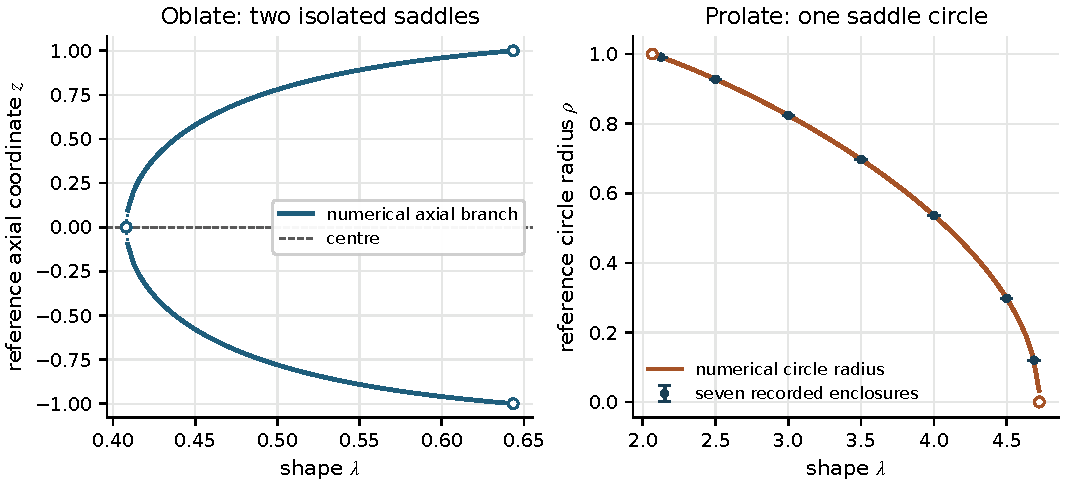
\includegraphics[width=\linewidth]{figures/branches.pdf}
\caption{参照座標において数値的に計算した、中心以外の
枝。左：扁平側の二つの軸上の鞍点。
右：扁長側のただ一つの停留円の半径。
右図に印を付けた七つの縦の区間は、
窓パッケージに記録された厳密な有理スライス包囲であり、その
幅はほとんどが描画の解像度より小さい。これらは
そのパッケージの証拠としての位置づけを引き継ぐ。白抜きの端点記号と点線の
接続は、分類された極限を示すものであり、追加の
数値的な根の計算を示すものではない。中心は全域で存続する。}
\label{fig:branches}
\end{figure}

図~\ref{fig:energy}のエネルギー断面では、
$128\times256$の球面則と$99\times99$の子午線格子を用い、
$q_1^2+q_3^2\leq0.98^2$を満たす7,525個の点を残した。
外縁の小さな部分を省いてあるので、有限解像度の画像が、
境界トレースが標本化によって確立されたかのように示唆することはない。
各パネルはそれぞれ固有のエネルギー尺度をもつ。扁長側の円の領域では、
子午線平面内の二つの十字は、一つの連結な
停留円との交点であり、二つの孤立した停留点ではない。

\begin{figure}[tbp]
\centering
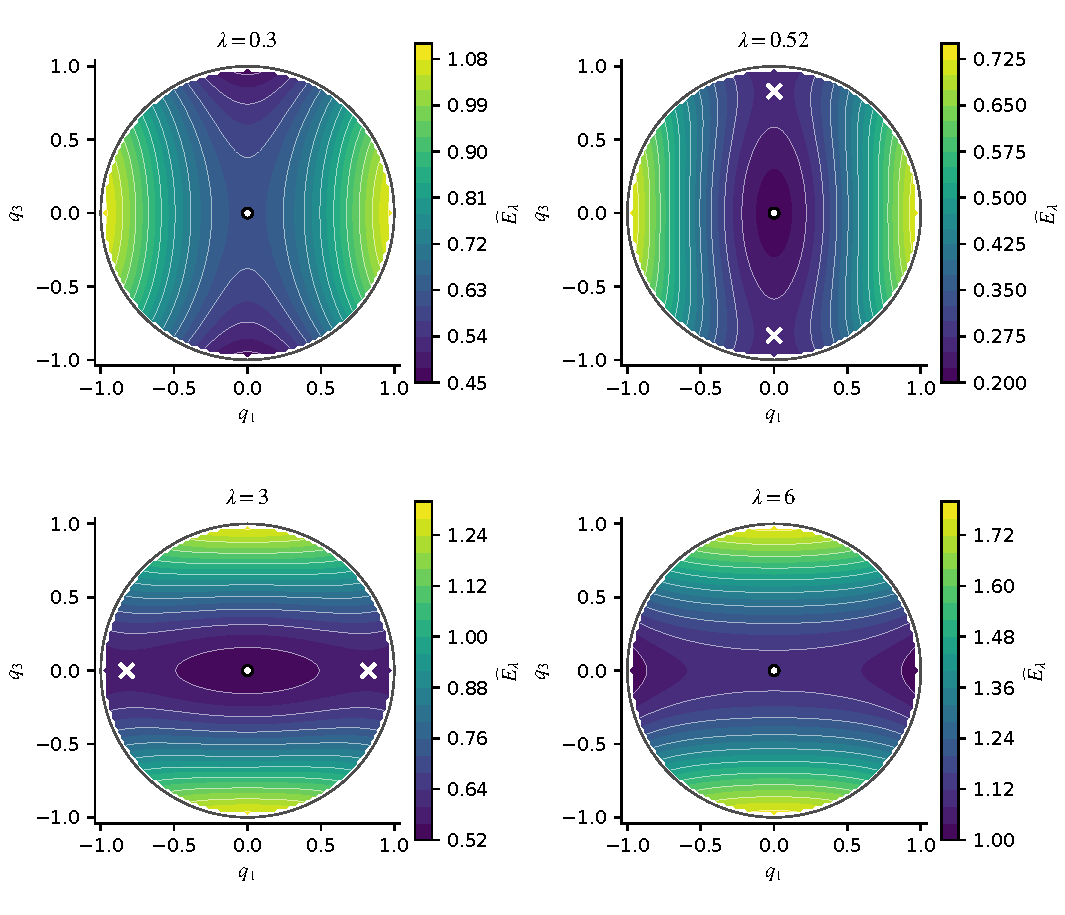
\includegraphics[width=.96\linewidth]{figures/energy_sections.pdf}
\caption{$\lambda=0.3,0.52,3,6$に対する$\widehat E_\lambda$の
参照座標での子午線断面。白い円板は中心を示し、白い十字は
中心以外の停留交点を示す。四つのパネルは
順に、中心の鞍点、中心の極小と
軸上の鞍点対、中心の極小と鞍点円、および
指数2の中心の鞍点を示す。各パネルの周りに描いた円は
参照境界であり、エネルギーは
半径$0.98$までしか標本化していない。これらは区間演算によらない数値的な図示である。}
\label{fig:energy}
\end{figure}

\subsection{記録された符号の余裕の大きさ}

定数$16189/2^{36}$と$3341881/2^{36}$は、
パラメータと空間の箱全体にわたる区間包囲から得られる、
小さな正の残余の余裕である。これらは
$V$の実際の大域的最小値の推定値ではなく、報告の単位$2^{-36}$は
包囲の誤差全体を測るものでもない。
繰り返し現れる変数の間の依存性、角度の値域の過大評価、および外側の箱の
幅は、いずれも符号の余裕の大部分を消費しうる
\citep{Rump2010}。C4の二つの縦方向の窓について、報告された$E_{zz}$と$E_z$の箱全体での余裕は、それぞれおよそ$1.75\times10^{-4}$と$4.86\times10^{-5}$である。別個の数値的な検討では、それぞれの窓で標本上の最小値が$1.07$と$0.32$の近くにあると報告された。この数桁の開きは包囲による損失を例示するものであり、標本上の最小値は連続体上の下界を与えない。尺度の比較として有用なのは、
$\rho=z=0.2$における直接の点値である：
\begin{center}
\begin{tabular}{rrr}
\toprule
$\lambda$&$V(0.2,0.2;\lambda)$&$H(0.2,0.2;\lambda)$\\
\midrule
1&1.261673&1.261673\\
1.5&1.810885&0.883353\\
2&2.053848&0.593574\\
3&2.169992&0.242475\\
5&2.025279&$-0.042247$\\
\bottomrule
\end{tabular}
\end{center}
求積則を$128\times256$から$256\times512$へ倍にしても、
これらの点値の変化は高々$1.65\times10^{-14}$である。
この一致は桁を認証するものではなく、
連続体上の下界を与えるものでもない。これは、記録された下端が非常に小さくても、
典型的な内点で導関数がほとんど消えていることを
必ずしも意味しない理由を例示するにすぎない。

\subsection{軸方向の凹性の拡張の可能性}

解析的な凹性の補題は、
$0<\lambda\leq1/32$に対する一様評価を証明する。符号に関する次のより強い言明が成り立てば、
残りの扁平側の解析の多くが簡単になる。

\begin{conjecture}\label{conj:concavity}
すべての$0<\lambda<\cO$と$|q|<1$に対して、
\[
 \partial_{zz}\widehat E_\lambda(q)<0.
\]
\end{conjecture}

$96\times192$の球面則による数値的な確認では、
$\lambda=1/16,1/8,1/4,0.35,0.4,0.4079$のそれぞれについて、
半径$0.96$の非負の子午線四分円板内の
473個の点を標本とした。
標本値はすべて負であった。これらの有限
標本における最大値は、それぞれおよそ
$-0.223524,-0.367927,-0.328099,-0.138342,-0.019734$、
および$-0.000147$であった。
さらに、境界に近い八つの弧のそれぞれの上で、等間隔な17個の子午線角において弦Hessianの求積を行ったところ、標本値はすべて狭義に負であった。$\lambda=1/128,1/64,1/32$に対しては半径$0.9999$を用いた。$\lambda=0.25,0.35,0.4,0.4079,0.42$に対しては$0.9995$を用いた。二つの組において、負の度合いが最も小さい標本値は、それぞれおよそ$-0.031$と$-0.487$であった。これらは点ごとの診断である。とくに、$0.42>\cO$は予想の範囲外にあり、そこでは中心がすでに正の軸方向曲率をもつ。

最大値がつねに中心でとられるという主張は
より強いものであり、すべての標本がそれを示唆しているわけではない：
$\lambda=1/8$では、$(\rho,z)=(0.88,0)$における値はおよそ
$-0.367927$であり、中心での値$-0.383316$より大きい。
$1/4$から$0.4079$までの四つの標本パラメータについては、
標本上の最大値は確かに中心でとられる。
予想~\ref{conj:concavity}は
最大値の位置についての主張を含まず、本節のいかなる計算も、
既存の証明義務を取り除くためには用いていない。

\subsection{三軸に関する具体的な問題}

$\lambda$を$(\bP,\cP)$の真に内側に固定し、
$M_\lambda$を次で置き換えて回転対称性を破る：
\[
 M_{\lambda,\epsilon}
 =\diag(e^\epsilon,e^{-\epsilon},1)M_\lambda.
\]
その行列式は1のままである。停留円の
分類を仮定すると、摂動前の円に沿う法方向のHessianは
可逆である。したがって陰関数定理により、
その円の近くで二つの法方向の臨界方程式が解かれ、
残りの方程式は周期的な角度エネルギー
$\Psi_\epsilon(\phi)$に帰着される。
第一変分は
$T=\diag(1,-1,0)$について線形である。このテンソルを$\phi$だけ回転すると、
角度の重み2の余弦成分と正弦成分が生じ、
$q_2=0$に関する鏡映により、$(\rho_*,0,0)$における正弦成分は
消える。法方向の補正の一次の寄与は、
摂動前の勾配が零であるため消える。
したがって、
$A(\lambda)=\left.\partial_\epsilon
\widehat E_{\lambda,\epsilon}(\rho_*,0,0)\right|_{\epsilon=0}$とおくと、
簡約された展開は
\[
 \Psi_\epsilon(\phi)
 =\Psi_0+\epsilon A(\lambda)\cos(2\phi)
   +O_{C^2(S^1)}(\epsilon^2),
\]
となる（ただし$A(\lambda)\ne0$とする）。
十分小さい零でない$\epsilon$に対して、主要項の角度微分の四つの単純
零点は存続し、近くの臨界点を
尽くす。一意的な法方向の解に引き継がれる座標鏡映により、
それらは正確に
$\phi=k\pi/2$に、すなわち向かい合う二組の主軸上の対に位置する。
それらの角度方向の曲率は符号が交互に変わる。法方向のHessianのSchur補行列は、
簡約された角度方向の曲率との合同なブロック分解を
与える。二つの法方向の
曲率は互いに逆の符号を保つので、それらの点のうち二つは
Morse指数1をもち、二つは指数2をもつ。

厳密な角度方程式もある。正定値行列$C=L^TL$に対してエネルギーを$F(C,q)$と書き、対称行列$G$を$D_CF[U]=\operatorname{tr}(GU)$によって定める。半軸$\ell_i$をもつ主軸枠において$T_{ij}=2\ell_i\ell_jG_{ij}$とおく。任意の回転$R$に対して、参照積分変数の変換により$F(RCR^T,Rq)=F(C,q)$が成り立つ。$(1,2)$平面内の回転について微分すると、次を得る：
\[
 q_1E_2-q_2E_1=(\ell_2/\ell_1-\ell_1/\ell_2)T_{12}.
\]
同様に、上に示した対角変形の微分から、第一軸上の摂動前の円の点において$A=T_{11}-T_{22}$が得られる。この厳密な恒等式は、零でない変形においても成り立つ。

$\cP$の近くの固定した形状に対して、第一軸上の形状微分は$\rho$について滑らかで偶である。その定数項は、二つの赤道軸の入れ替えにより消える。よって、円が縮むとき$A=O(\rho_*^2)$である。一様に評価すべき自然な量は$A/\rho_*^2$である。通常の求積によると、$\lambda=2.1,3,4,4.7$においてそれぞれ$0.6744,0.5744,0.4879,0.4399$となる。枝全体における正の一様下界は、ここでは未解決の評価として残る。序論で引用した局所的な三軸の研究は、扁長側の中心遷移の近傍に関するものである。これら四つの標本も、厳密な角度方程式それ自体も、三軸族全体にわたって他の臨界点を排除するものではない。

\section{入手先、再現性、および草稿の状況}
\label{sec:availability}

計算に関する参照文献は、
公開リポジトリ\texttt{cotaxxxx/bg-spheroid-family}および
\texttt{cotaxxxx/bg-oblate-spheroid}内の固定されたコミットとパスを特定する。
それ以前の背景資料は公開リポジトリ
\texttt{cotaxxxx/basepoint-geometry}にある。扁平の極限の解析的な
議論と、扁長側の裾の議論のうち軸上の部分は、
固定された研究記録をもとに、ここで詳しく展開したものである
\citep{data-oblate-analytic,data-prolate-axis}。
球の場合の証明は第~\ref{sec:sphere}節で与えており、
未公表の球に関する原稿を必要としない。
記録V24（2026年11月16日）：\texttt{cotaxxxx/bg-spheroid-family}、
コミット\texttt{127be52046e9498d1306fe3d35c3e02e91c636de}、
ファイル\href{https://github.com/cotaxxxx/bg-spheroid-family/blob/127be52046e9498d1306fe3d35c3e02e91c636de/runs/2026-11-16/D_OB_GLOBAL_CLOSED_V24/JUDGE_RULING_D_OB_GLOBAL_CLOSED_20261116.md}{\path{JUDGE_RULING_D_OB_GLOBAL_CLOSED_20261116.md}}%
（日本語の作業記録）。この一次記録の正確な写しは、
付属のソース一式の\path{provenance/V24/}以下に含まれている。
付属のプロジェクト水準のAI監査は、組み立ての議論と
出典の参照を点検した。選ばれた区間箱の計算は
独立に再計算され、厳密な整数被覆検査が
\path{CURRENT_REPRODUCTION_v0_5_4.md}に記録された範囲で行われたが、
この監査もそれらの検査も、C1--C6の完全な再実行には当たらない。

主張ごとの再現の対応表については、ソース一式内の
\path{CURRENT_REPRODUCTION_v0_5_4.md}を見よ。これは、
C1--C6を、固定された入力パッケージ、生成および検査のコマンド、
台帳のパス、独立な再評価の範囲とともに、
残してある過去の\path{REPRODUCTION.md}とは別に列挙する。この新しい対応表は、
列挙された元の生成プログラムがすべて再実行されたとも、
その元の解析的な核が独立に再導出されたとも主張しない。

付属の改訂版一式には、原稿のソース、
文献データ、ベクター形式の図、図のデータと再現用スクリプト、
および固定された計算ソースの対応表が含まれる。これは、
すべての上流の計算についての完全な認証済みアーカイブではない。
そのような統合された証明パッケージに対するアーカイブ用DOIは、
この改訂版では主張しない。固定されたリリースには、厳密な
入力の箱、選ばれたすべての最終の葉、係数表、
生成プログラムと検査プログラムのソース、ビルド環境、実行
コマンド、およびファイルのハッシュを、C1--C6から
対応する受理済みの記録への直接の対応表とともに含めるべきである。

互いに異なる三つの義務、すなわち解析的な
核の正しさ、その実装における正しい外向き演算と誤差上界、
および分類で用いる領域被覆の
完全性がある。ファイルのハッシュが確立するのは同一性であって、
これらの数学的性質のいずれでもない。元の
核による再現と、別途導出した核による再評価とは、
異なる失敗の様式に対処する。完全に独立な数値的再実行は
ここでは主張せず、その現在の範囲は
第~\ref{subsec:computational-workload}節に述べてある。
補足資料は、再実行のコマンド、固定された所在、および選択規則を与える。ソース一式には、独立な区間計算とそれらの整数被覆検査が含まれる。

\paragraph{AIツールの使用。}
ChatGPT（OpenAI）は、探索的な導出、数値計算
コードと検証スクリプト、英語の文言の提案、
改稿、および組版を補助した。Codex（OpenAI）はコーディングと
原稿の検討を補助し、GPT-6.2 Astra（OpenAI）は研究設計と
専門的な計算作業を補助した。Claude（Anthropic）は、
議論の組み立て、出典の参照、および原稿の差分について、別個のプロジェクト水準のAI監査を
行い、Claude Code（Anthropic）は、記録された範囲で特別なコード
監査と独立な検査を提供した。Muse（Meta）は、
扁平側のD5の作業の一部を含む、選ばれた計算
資料について、追加の外部AI監査を行った。これらの記録は、
C1--C6の独立に実装された完全な再実行でも、外部の
人間による査読でもない。英語の初稿の段落と、
その後の翻訳または校正とを区別する来歴は、まだ完全には
再構成されておらず、したがって、「校正」に限定した説明は
主張しない。ソース一式にはAI来歴の検討記録が含まれる。
投稿先候補の学術誌の初稿に関する制限への適合は
主張しない。提案されたすべての主張、
文献、コードの寄与、および最終的な開示についての著者による検証は未了である。

\begingroup
\interlinepenalty=10000
\bibliographystyle{plainnat}
\bibliography{references,references_additions,references_computation}
\endgroup
\end{document}
